\documentclass[a4paper, 8pt]{extarticle}
\setcounter{page}{0}
\renewcommand{\baselinestretch}{1} %spacing between lines

\usepackage{verbatim} %multiline comments


%generate geometry of paper
\usepackage[landscape]{geometry}
\geometry{
     %total={210mm,297mm},
     left=2mm,
     right=2mm,
     top=15mm,
     bottom=-1mm,
 }
\usepackage[utf8]{inputenc}
\usepackage[normalem]{ulem}

\usepackage{amssymb}
\usepackage{amsmath}
\usepackage{amsfonts}
\usepackage{bm}

\usepackage{mathtools}
\usepackage[ngerman]{babel}

\usepackage{multicol} %multiple columns
\usepackage{wrapfig} %wrap text around figures


%get rid of spacing between lists
\usepackage{enumitem} 
    \setlist{nolistsep}

%custom header with title & authors
\usepackage{fancyhdr} 
    \pagestyle{fancy}
    \fancyhf{}
    \rhead{Joshua Näf, \textit{naefjo@ethz.ch}; Franz Bühlmann, \textit{franzbu@ethz.ch}}
    \lhead{\textbf{Dimensionieren I HS19, Prof. Dr. E. Mazza}}
    \setlength{\headsep}{1mm}
    \chead{\textbf{\thepage}}


%imagepackage
\usepackage{graphicx} 
    \graphicspath{ {./images/} }

\usepackage{parskip} %Einzug aus, Absatzabstand ein
    \tolerance=2000 %Toleranz für Wortzwischenräume
    \setlength{\emergencystretch}{20pt} %Zusätzliche Zeilendehnbarkeit in Notfällen
    \setlength\parindent{0pt}
    \setlength{\columnseprule}{1px} %thickness of column seperator

%New Titles
\usepackage{tcolorbox}
    \definecolor{seccol}{RGB}{7, 61, 50}
    \definecolor{subseccol}{RGB}{29, 120, 116}
    \definecolor{subsubseccol}{RGB}{103, 146, 137}
% Section
\renewcommand{\section}[1]{
	\begin{tcolorbox}[
			arc=0mm,
			colback=seccol,
			colframe=white,
			bottomrule = 0 mm,
			toprule = 0 mm,
			leftrule = 0 mm,
			rightrule = 0 mm,
			valign=center,
			left=0.5mm,
			top= 0.2 mm,
			bottom= 0.2 mm,
			fontupper=\color{white},
			before skip = 2mm,
			leftright skip = -0.5mm,
			after skip = 0 mm]

		\textbf{#1}
	\end{tcolorbox}
}
	
% Subsection	
\renewcommand{\subsection}[1]{
	\begin{tcolorbox}[
			arc=0mm,
			colback=subseccol,
			colframe=white,
			bottomrule = 0 mm,
			toprule = 0 mm,
			leftrule = 0 mm,
			rightrule = 0 mm,
			valign=center,
			left=0.5mm,
			top=0.2mm,
			bottom=0.2mm,
			fontupper=\color{white},
			before skip = 0.5mm,
			leftright skip = -0.5mm,
			after skip = 0.5 mm]
			
		\small \textbf{#1:}
	\end{tcolorbox}
}
	
% Subsubsection	
\renewcommand{\subsubsection}[1]{
	\begin{tcolorbox}[
			arc=0mm,
			colback=subsubseccol,
			colframe=white,
			bottomrule = 0 mm,
			toprule = 0 mm,
			leftrule = 0 mm,
			rightrule = 0 mm,
			valign=center,
			left=0.5mm,
			top=-0.2mm,
			bottom=-0.2mm,
			fontupper=\color{white},
			before skip = 0.5mm,
			leftright skip = -0.5mm,
			after skip = 0.5 mm]
			
		\small \textbf{#1:}
	\end{tcolorbox}
}
\newcommand{\TODO}[1]{\large\textcolor{red}{\textbf{TODO: #1\\}}\normalsize}

\usepackage{stackengine,xcolor}
\def\cpm{\mathbin{\ensurestackMath{\abovebaseline[-3.4pt]{%
  \stackunder[-3.5pt]{\color{blue!70}+}{\color{red}-}}}}}

\title{Dimensionieren 1 Zusammenfassung}
\author{Joshua Näf, Franz Bühlmann}
\date{}

\begin{document}

\maketitle
\begin{center}
    This summary has been written based on the Lecture 151-0303-00L  Dimensionieren I by Prof. Dr. Mazza (HS19) and the Kolloquium by Dr. Raoul Hopf. There can be no guarantee that this summary will prove viable during the exercises or exam since the lecture has been redesigned from the ground up which resulted in this summary being a work in progress throughout the semester. There is also no guarantee for completeness and/or correctness regarding the content of this summary. Use it at your own discretion. All pictures are taken from either the lecture notes, the MechII summary by Nick Bührer or the WuFI/II Summary by Cédric de Crousaz.
    
    This is a WIP 
    \footnote{\label{foot:2}Version: 21.12.19}
\end{center}
\newpage
\begin{multicols*}{3}

\section{Methoden d Strukturanalyse}
    \subsection{Gleichungen des Kontinuums}
        \subsubsection{GGWB des Kontinuums}
            \small
            \[\sigma_{11,1} + \sigma_{12,2} + \sigma_{13,3} + f_1 = 0\]
            \[\sigma_{21,1} + \sigma_{22,2} + \sigma_{23,3} + f_2 = 0\]
            \[\sigma_{31,1} + \sigma_{32,2} + \sigma_{33,3} + f_3 = 0\]
            
        \subsubsection{Stoffgleichungen (SG)}
            %\vspace{-1mm}
            \[\varepsilon_{11} = \frac{1}{E}\lbrack\sigma_{11} - \nu(\sigma_{22} + \sigma_{33})\rbrack \quad \sigma_{11}=\frac{E}{1+\nu}\lbrack\varepsilon_{11}+\frac{\nu}{1-2\nu}(\varepsilon_{11}+\varepsilon_{22}+\varepsilon_{33})\rbrack\]
            %\vspace{-3mm}
            \[\varepsilon_{22} = \frac{1}{E}\lbrack\sigma_{22} - \nu(\sigma_{11} + \sigma_{33})\rbrack \quad \sigma_{22}=\frac{E}{1+\nu}\lbrack\varepsilon_{22}+\frac{\nu}{1-2\nu}(\varepsilon_{11}+\varepsilon_{22}+\varepsilon_{33})\rbrack\]
            %\vspace{-1mm}
            \[\varepsilon_{33} = \frac{1}{E}\lbrack\sigma_{33} - \nu(\sigma_{22} + \sigma_{11})\rbrack \quad \sigma_{33}=\frac{E}{1+\nu}\lbrack\varepsilon_{33}+\frac{\nu}{1-2\nu}(\varepsilon_{11}+\varepsilon_{22}+\varepsilon_{33})\rbrack\]
            \[\varepsilon_{12}=\frac{\tau_{12}}{2G}; \qquad 2G=\frac{E}{1+\nu}\]
            
        \subsubsection{Kinematische Randbedingungen (KR)}
            \[\varepsilon_{11} = u_{1,1}\qquad\qquad\varepsilon_{22} = u_{2,2}\qquad\qquad\varepsilon_{33} = u_{3,3}\]
            \[\varepsilon_{12} = \frac{1}{2}(u_{1,2} + u_{2,1});\quad\varepsilon_{13} = \frac{1}{2}(u_{1,3} + u_{3,1});\quad\varepsilon_{23} = \frac{1}{2}(u_{2,3} + u_{3,2})\]
            \normalsize
            \begin{comment}
                \[\varepsilon_{11} = u_{1,1}\quad\quad\quad\quad\varepsilon_{12} = \frac{1}{2}(u_{1,2} + u_{2,1})\]
                \[\varepsilon_{22} = u_{2,2}\quad\quad\quad\quad\varepsilon_{13} = \frac{1}{2}(u_{1,3} + u_{3,1})\]
                \[\varepsilon_{33} = u_{3,3}\quad\quad\quad\quad\varepsilon_{23} = \frac{1}{2}(u_{2,3} + u_{3,2})\]
            \end{comment}
        
    

\section{Balken}
    \subsection{Formulierungen}
        2 Möglichkeiten: Statische Formulierung und Kinematische Formulierung.\\
        Statische Formulierung: GGB \& SG erfüllt, KR zum Teil nicht. Generell zu weich.\\
        Kinematische Formulierung: GGB \& SG nicht erfüllt, KR schon. Steifer als echt. Schlechte approx mit nur einer Funktion. Approximation wird besser durch besseren Ansatz und mehrere Elemente.
    \subsection{Energiesätze}
        \subsubsection{Definitionen}
            \begin{itemize}
                \item Spannungsfeld $\sigma_{ij}(x,y,z)$ zulässig falls: GGB \& \textit{stat} RB erfüllt.
                \item Verschiebungsfeld $u_i(x,y,z)$ zulässig falls: stetig \& \textit{kin} RB erfüllt (schwächere Bedingung).
                \item Verschiebungsfeld \& Spannungsfeld verträglich iff SG erfüllt.
                \item Deformationsenergie: $U=\frac{1}{2}\iiint_V \sigma_{ij}\cdot\varepsilon_{ij}dV$
                \item Potential äussere Energie:\\
                $V=-\iiint_V f_i\cdot u_idV-\sum_{a}\underline{F}_a\cdot\underline{u}_a$
                \item Potentielle Energie: $E_p=U+V$
                \item Komplementäre Deformationsenergie:\\ $U_K=\iiint_V(\oint_0^{\sigma_{ij}}\varepsilon_{ij}d\sigma_{ij})dV := U$  (lin. elast.)
            \end{itemize}
            
        \subsubsection{Satz vom Minium der potentiellen Energie (SMPE)}
            Aus der Menge der zulässigen Verschiebungsfelder $u_i^*(x,y,z)$ \& der damit verträglichen Spannungsfelder $\sigma_{ij}^*(x,y,z)$ macht das wirkliche Verschiebungsfeld $u_i(x,y,z)$ $E_P$ minimal. $E_p(u_i) < E_p(u_i^*)$\\\\
            \textit{Direkte Anwendung:} Ansatz für $u_i(x,y,z,a_\gamma)$, zulässig (stetig, KRB erfüllt). Berchene $\varepsilon_{ij}^*$ (aus KR) und verträgliche Spannungen $\sigma_{ij}^*$ (aus SG). $\sigma_{ij}^*$ braucht nicht zulässig zu sein (GGB \& SRB evtl. nicht erfüllt). Berechne $E_p(u_i^*)$ und bestimme $a_\gamma$ mit $\frac{\partial E_p}{\partial a_\gamma}=0$.
            
        \subsubsection{Satz vom Min. der kompl. Deform-energie (SMkDE)}
            Aus der Menge der zulässigen Spannungsfelder $\sigma_{ij}^*(x,y,z)$ \& damit verträglichen $\varepsilon_{ij}^*(x,y,z)$ macht das wirkliche Spannungsfeld $\sigma_{ij}(x,y,z)$ die komplementäre Deformationsenergie $U_K$ minimal. $U_K(\sigma_{ij}) < U_K(\sigma_{ij}^*)$\\\\
            \textit{Direkte Anwendung:} Ansatz für $\sigma_{ij}^*(x,y,z,a_\gamma)$, zulässig (GGB, SRB erfüllt). Berechne $\varepsilon_{ij}^*$ (aus SG), nicht unbedingt zulässig (KR, KRB eventuell nicht erfüllt). Berechne $U_K(\sigma_{ij}^*)$ und bestimme $a_\gamma$ mit $\frac{\partial U}{\partial a_\gamma}=0$.
            
        \subsubsection{Bsp}
            Ansatz:\\
            $u_y=ax^3+bx^2; \quad u_x=-\frac{du_y}{dx}y= -(3ax^2+2bx)y; \quad u_z = 0$\\
            KR: $\varepsilon_{xx} =(-6ax-2b)y; \quad \varepsilon_{yy}=\varepsilon_{zz}=\varepsilon_{xy}=\varepsilon_{yz} = \varepsilon_{xz}=0$\\
            SG: $\sigma_{xx} = \alpha(-6ax-3b)y; \quad \sigma_{xy}=\sigma_{xz}=\sigma_{yz}=0$\\ $\sigma_{yy}=\sigma_{zz}=2G\frac{\nu}{1-2\nu}(-6ax-2b)y$\\
            SMPE:\\
            $U=\frac{1}{2}\int_0^l\int_\frac{-h}{2}^\frac{h}{2}\int_{-\frac{b}{2}}^\frac{b}{2}(\sigma_{xx}\cdot\varepsilon_{xx})dzdydx=6\cdot\alpha\cdot I\cdot l(\alpha^2l^2+\frac{b^2}{3}+abl)$\\
            $V=-P\cdot u_y(x=l)=-P(al^3+bl^2)$\\
            $E_p=6\alpha Il(a^2l2+\frac{b^2}{3}+abl)-P(al^3+bl^2)$
            \vspace{-3mm}
            \small\[\frac{\partial E_p}{\partial a} = 0 \Rightarrow a=-\frac{P}{6\alpha I};\quad\frac{\partial E_p}{\partial b} = 0 \Rightarrow b=-\frac{P}{2\alpha I}\]\normalsize
        \vspace{-3mm}    
        \subsubsection{SMPE \& FEM}
            \begin{wrapfigure}[5]{r}{0.4\linewidth}
                \vspace{-5mm}
                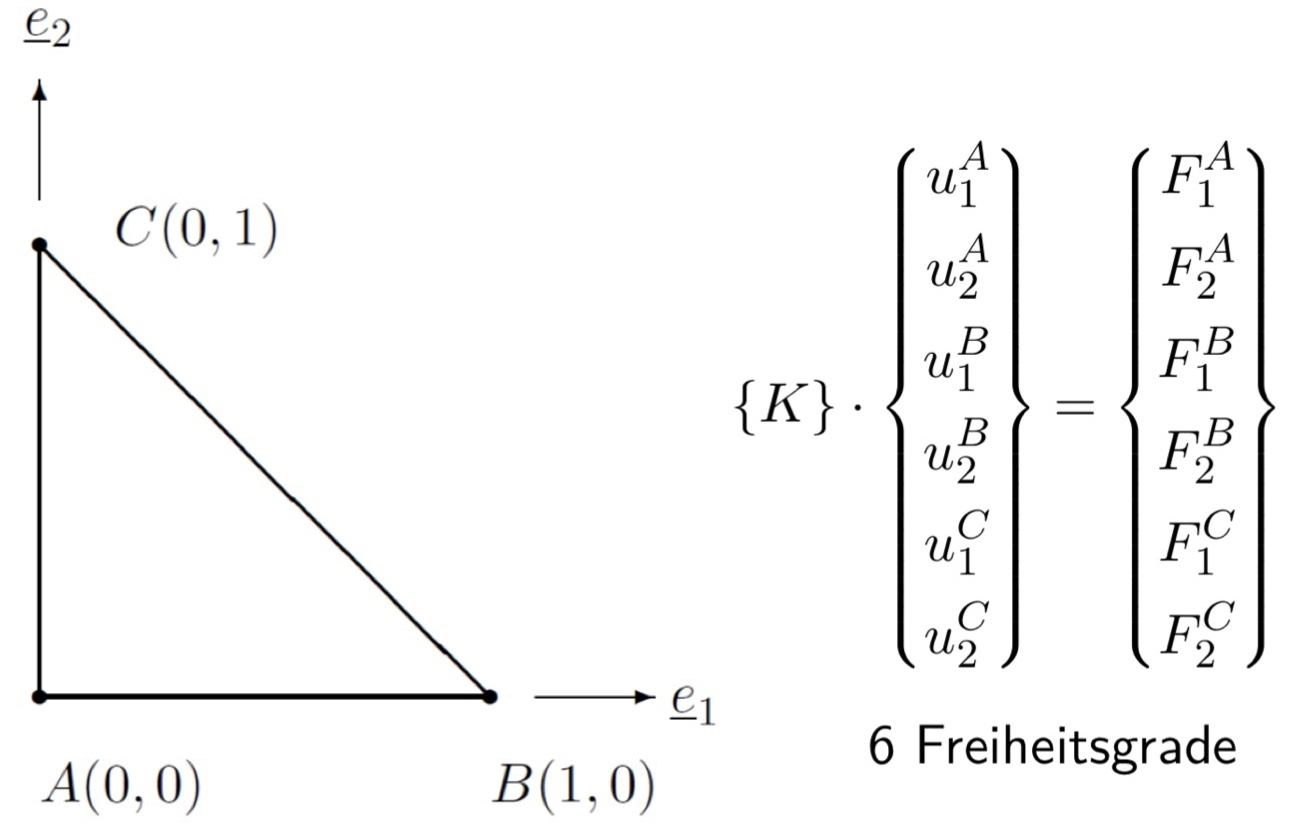
\includegraphics[width=\linewidth, height=23mm]{02/Dreieckselement}
            \end{wrapfigure}
            Relation der Verschiebungsfreiheitsgrade der Knoten ($\{u\}$) und äusseren Kräften an den Knoten ($\{F\}$) über die globale Steifigkeitsmatrix ($\{K\}\in\mathbb{R}^{6\times6}$): $\{F\}=\{K\}\{u\}$
            
        \subsubsection{Bsp}
            $u_1=ax_1+bx_2+c$; $u_2=dx_1+ex_2+f$\\
            $\Rightarrow u_1(x_1=0,x_2=0)=c=u_1^A$; $\quad u_2(x_1=0,x_2=0)=f=u_2^A$;...\\
            $\Rightarrow u_1=(u_1^B-u_1^A)x_1+(u_1^C-u_1^A)x_2+u_1^A$;\\
            \small$u_2=(u_2^B-u_2^A)x_1+(u_2^C-u_2^A)x_2+u_2^A$\normalsize\\
            $\varepsilon_{11}=(u_1^B-u_1^A)$; $\varepsilon_{22}=(u_2^C-u_2^A)$; $\varepsilon_{12}=\frac{1}{2}(u_2^B-u_2^A+u_1^C-u_1^A)$
            $\Rightarrow\sigma_{ij}(u_1^A,...,u_2^C,E,\nu)$ (aus KR)\\
            $U=\frac{1}{2}\cdot\frac{1}{2}(\sigma_{11}\cdot\varepsilon_{11}+\sigma_{22}\cdot\varepsilon_{22}+2\sigma_{12}\cdot\varepsilon_{12})\cdot t$ mit Dicke $t$ und Fläche $\frac{1}{2}$.\\
            $V=-(F_1^A\cdot u_1^A+F_2^A\cdot u_2^A+...+F_2^C\cdot u_2^C)$\\
            $E_p=U+V=E_p(u_1^A,...,u_2^C,E,\nu,t)=\alpha_1(u_1^A)^2+\alpha_2u_1^Au_1^B+ ...-(F_1^Au_1^A+...)$\\
            Minimum $E_p:$ $\frac{\partial E_p}{\partial u_i^\kappa}=0$ mit $i=1,2$ \& $\kappa=A,B,C$ (6Gl)\\
            Bsp: $\frac{\partial E_p}{\partial u_1^A}=\frac{\partial U}{\partial u_1^A}+\frac{\partial V}{\partial u_1^A}$ (lin. Fkt. in $u_1^A,..,u_2^C$) \\$\Rightarrow F_1=\kappa_{11}u_1^A+...+\kappa_{16}u_2^c$; $\kappa_{11},...,\kappa_{16}$: 1. Zeile von $\{K\}$

\section{Scheibe}
    \subsection{Definition}
        \begin{wrapfigure}[7]{r}{0.5\linewidth}
            \vspace{-3mm}
            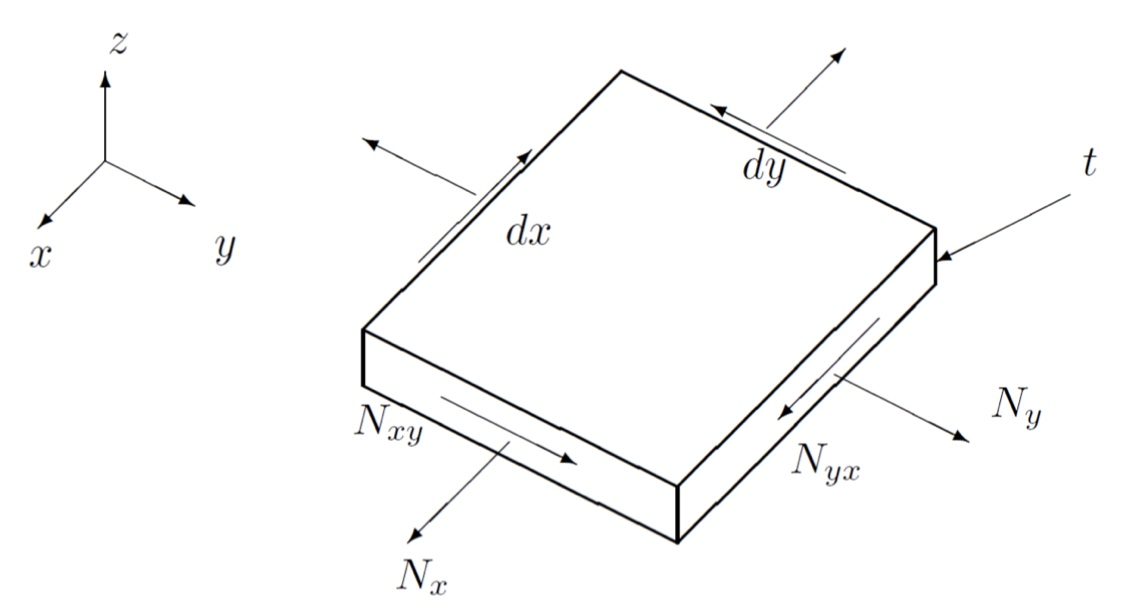
\includegraphics[width=\linewidth]{03/Scheibe}
        \end{wrapfigure}
        \textbf{Scheibenelement:} Dünnwandige Struktur mit Belastung in der Ebene. Äussere Kräfte dargestellt durch $N_x,N_y,N_{xy},N_{yx}$: Kräfte pro Längeneinheit ($\rightarrow$ Spannungen $\sigma_{xx},\sigma_{yy},\tau_{xy}$ über Dicke t integriert).

    \subsection{Annahmen}
        \begin{enumerate}[noitemsep]
            \item \textbf{Ebener Spannungszustand} ($\sigma_{zz},\tau_{xz},\tau_{yz}=0$)
            \item Übrige Spannungskomponenten sind konstant verteilt in z-Richtung (homogene Spannungsverteilung)
            \item Keine Volumenkräfte
            \item \textbf{Spannungsansatz} (GGB erfüllt)
        \end{enumerate}
        1, 2: Vernünftig, weil planare Dimensionen $\gg$ t \& keine Biegung. GGB reduziert sich zu: $\displaystyle\sigma_{xx,x} + \tau_{xy,y}=0$; $\sigma_{yy,y} + \tau_{xy,x}=0$
        $\rightarrow$Definiere $F(x,y)$ (Airy'sche Spannungsfkt) mit:\\ $\sigma_{xx}=F_{,yy}$; $\sigma_{yy}=F_{,xx}$; $\tau_{xy}=-F_{,xy}$.
        \\Aus Kompatibilitätsbedingung: $\varepsilon_{xx,yy}+\varepsilon_{yy,xx}=2\varepsilon_{xy,xy}$ \\$\rightarrow F_{,xxxx}+F_{,yyyy}+2F_{xxyy}=0 \Leftrightarrow\Delta\Delta F=0$.
        \\Funktion $F(x,y)$ so wählen, damit RB erfüllt.
	\\Da statischer Ansatz $\rightarrow$ Minimierung der komplementären Deformationsenergie.
    \subsection{Scheibe mit Loch}
        \begin{center}
            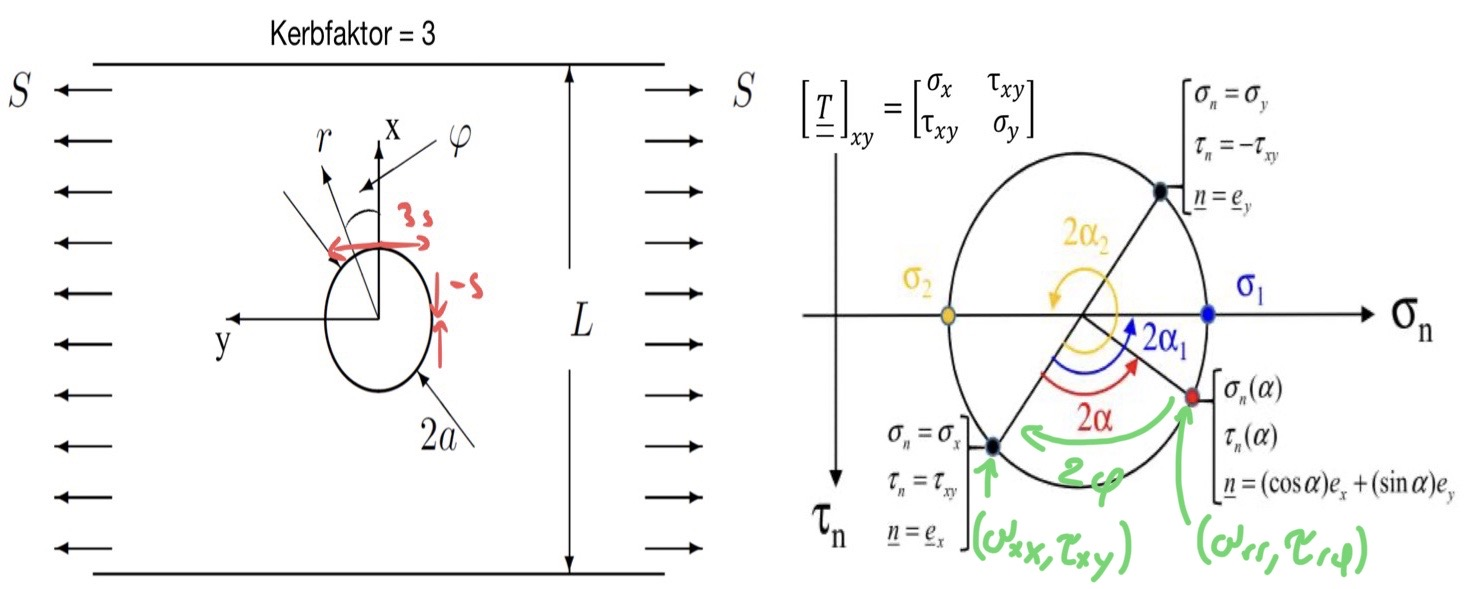
\includegraphics[width=0.9\linewidth, height=30mm]{03/mohr_and_loch_2.JPG}
            $\tiny{\lambda_{1,2}= \frac{1}{2}(\sigma_x+\sigma_y)\pm\sqrt{\frac{1}{4}(\sigma_x-\sigma_y)^2+\tau_{xy}^2}}$\\
            $\sigma_{\overset{\textcolor{blue}{rr}}{\textcolor{red}{\varphi\varphi}}}=\sigma_{xx}\overset{\textcolor{blue}{cos^2(\alpha)}}{\textcolor{red}{sin^2(\alpha)}}+\sigma_{yy}\overset{\textcolor{blue}{sin^2(\alpha)}}{\textcolor{red}{cos^2(\alpha)}} \cpm 2\tau_{xy}sin(\alpha)cos(\alpha)$\\
            $\tau_{r\varphi}=(\sigma_{yy}-\sigma_{xx})sin(\alpha)cos(\alpha)+\tau_{xy}(cos^2(\alpha)-sin^2(\alpha)$
        \end{center}
\columnbreak
        \begin{itemize}
            \item Lochradius a $\ll$ L
            \item Belastung durch uniforme, einachsige Spannung S in grosser Entfernung vom Loch
            \item Spannungsfreie Rissflanken ($r = a; \forall\varphi\in\mathbb{R} $): $\sigma_{rr}=0, \tau_{r\varphi}=0$
        \end{itemize}
        \textbf{Superposition} von mehreren Spannungen \& Spannungsrichtungen möglich.Schubspannungen in Hauptspannungen umwandlen.
        \begin{center}
            $\sigma_{\overset{\textcolor{blue}{\varphi\varphi}}{\textcolor{red}{rr}}}=\frac{s}{2}\left(1\cpm\frac{a^2}{r^2}\cpm cos(2\varphi)\left(1+3\frac{a^4}{r^4}\textcolor{red}{-4\frac{a^2}{r^2}}\right)\right)$
            $\tau_{r\varphi}=\frac{s}{2}\left(1-3\frac{a^4}{r^4}+2\frac{a^2}{r^2}\right)sin(2\varphi)$
        \end{center}

    \subsection{Scheibe mit Riss}
        Spannungsfreie Rissflanken ($\forall r, \varphi=\pm\pi$): $\sigma_{\varphi\varphi}=0, \tau_{r\varphi}=0$
        \begin{center}
            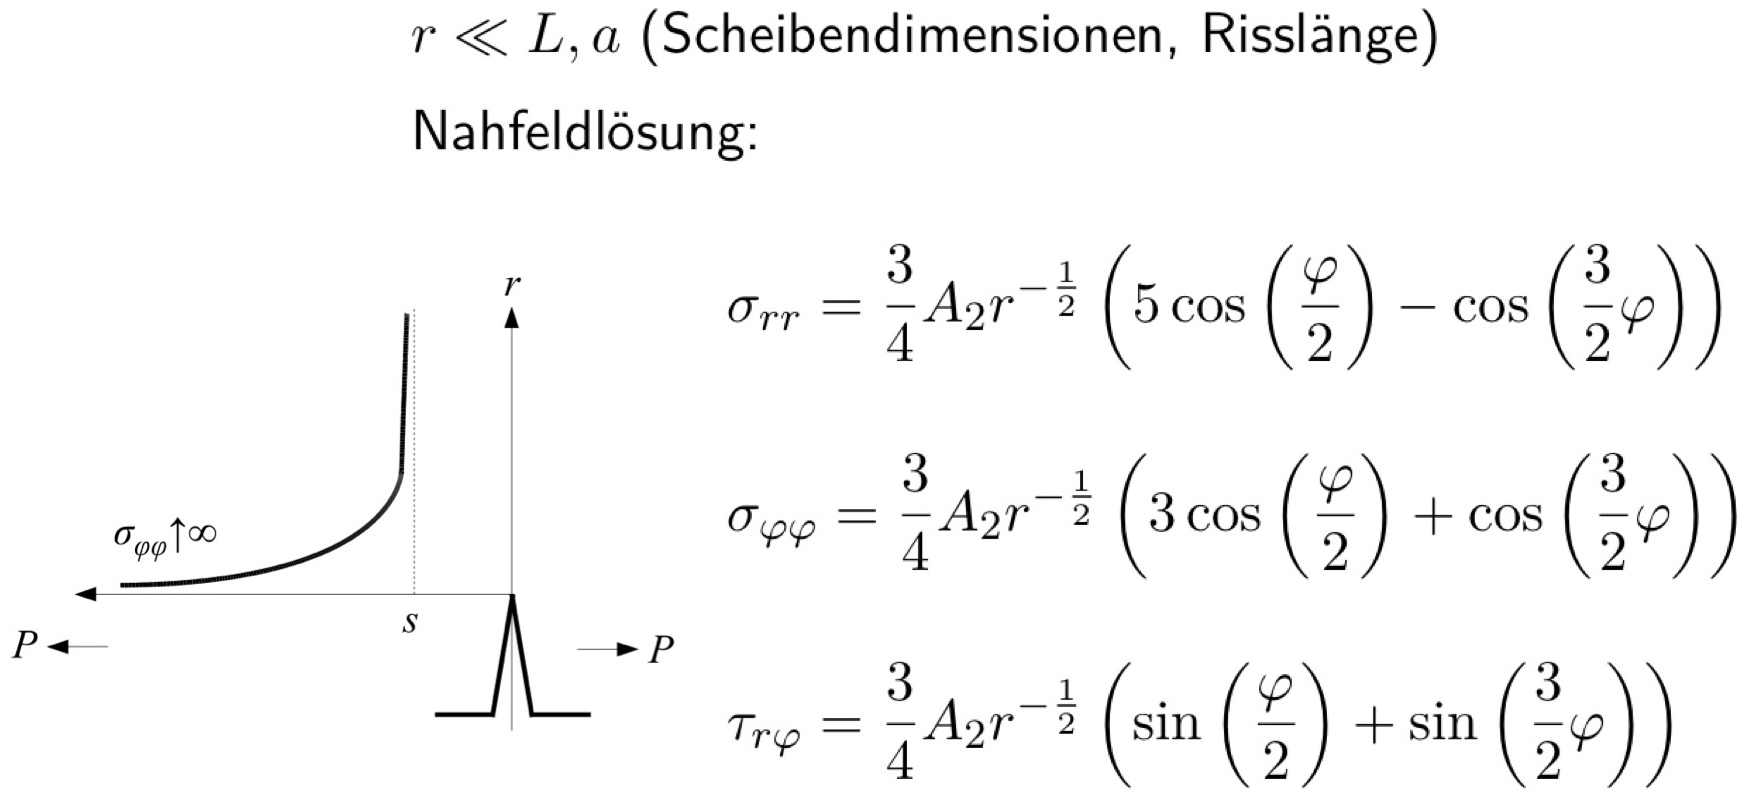
\includegraphics[width=70mm, ]{03/Scheiberiss}
        \end{center}
\vspace{-2mm}


\vspace{-3mm}
\section{Materialverhalten}{}
    \subsection{Festigkeitshypothesen}
        \subsubsection{Fliessbedingung/Fliessfunktion $\Phi(\sigma)$}
            Fliessbedingung: $\Phi(\sigma)<0$ (elastisch), $\Phi(\sigma)=0$ (plastisch)
            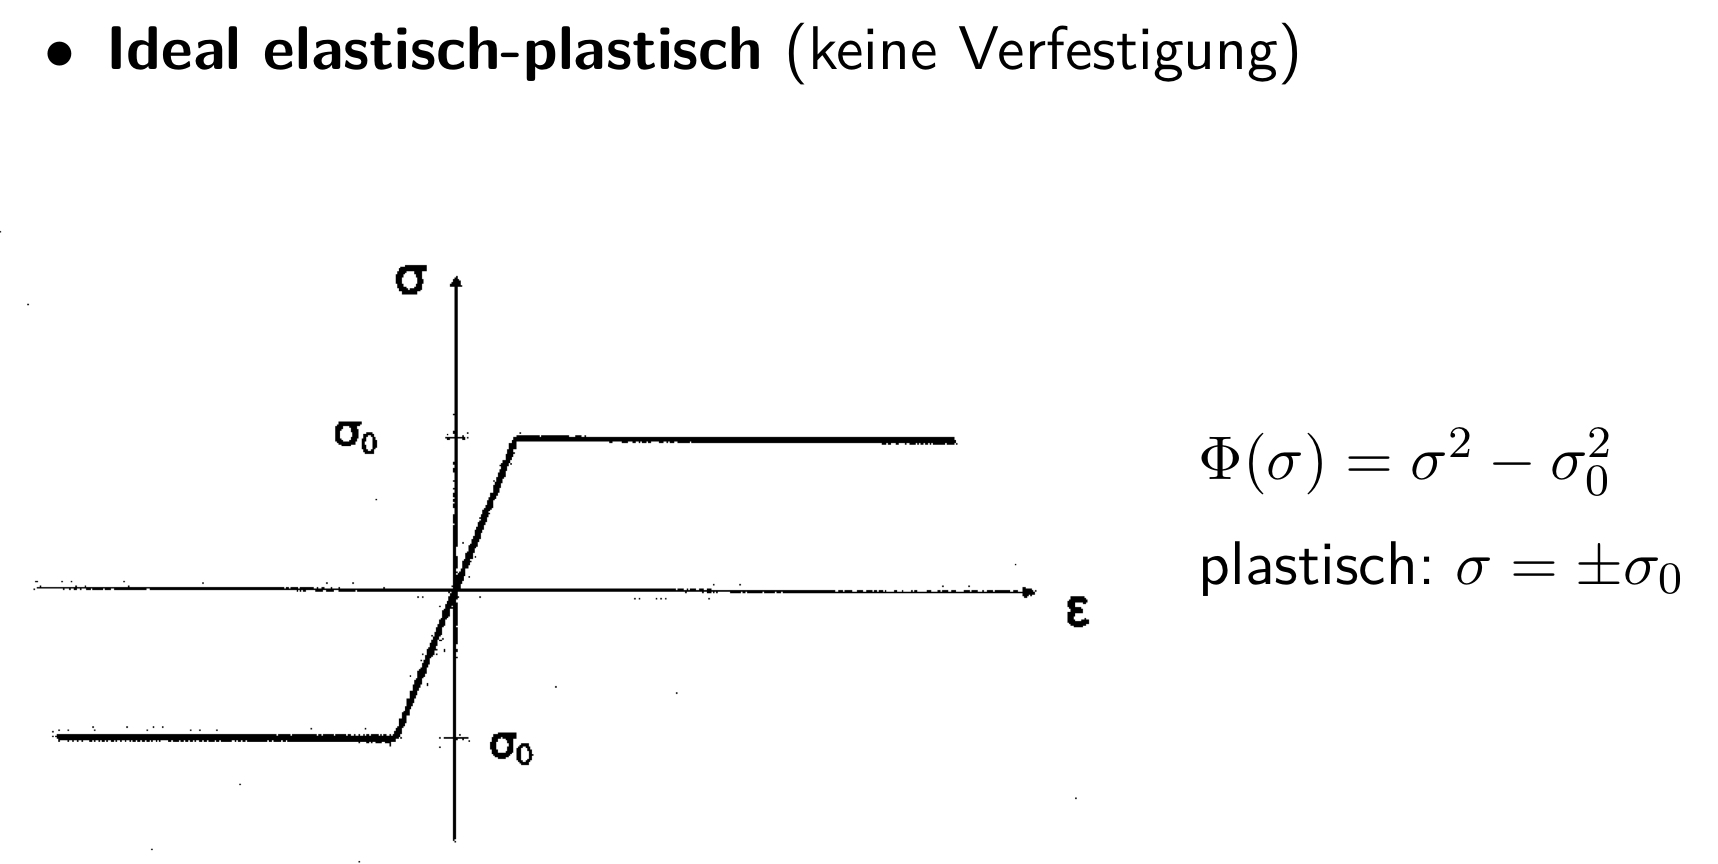
\includegraphics[width=0.5\linewidth]{04/Verf_ideal_elpl}
            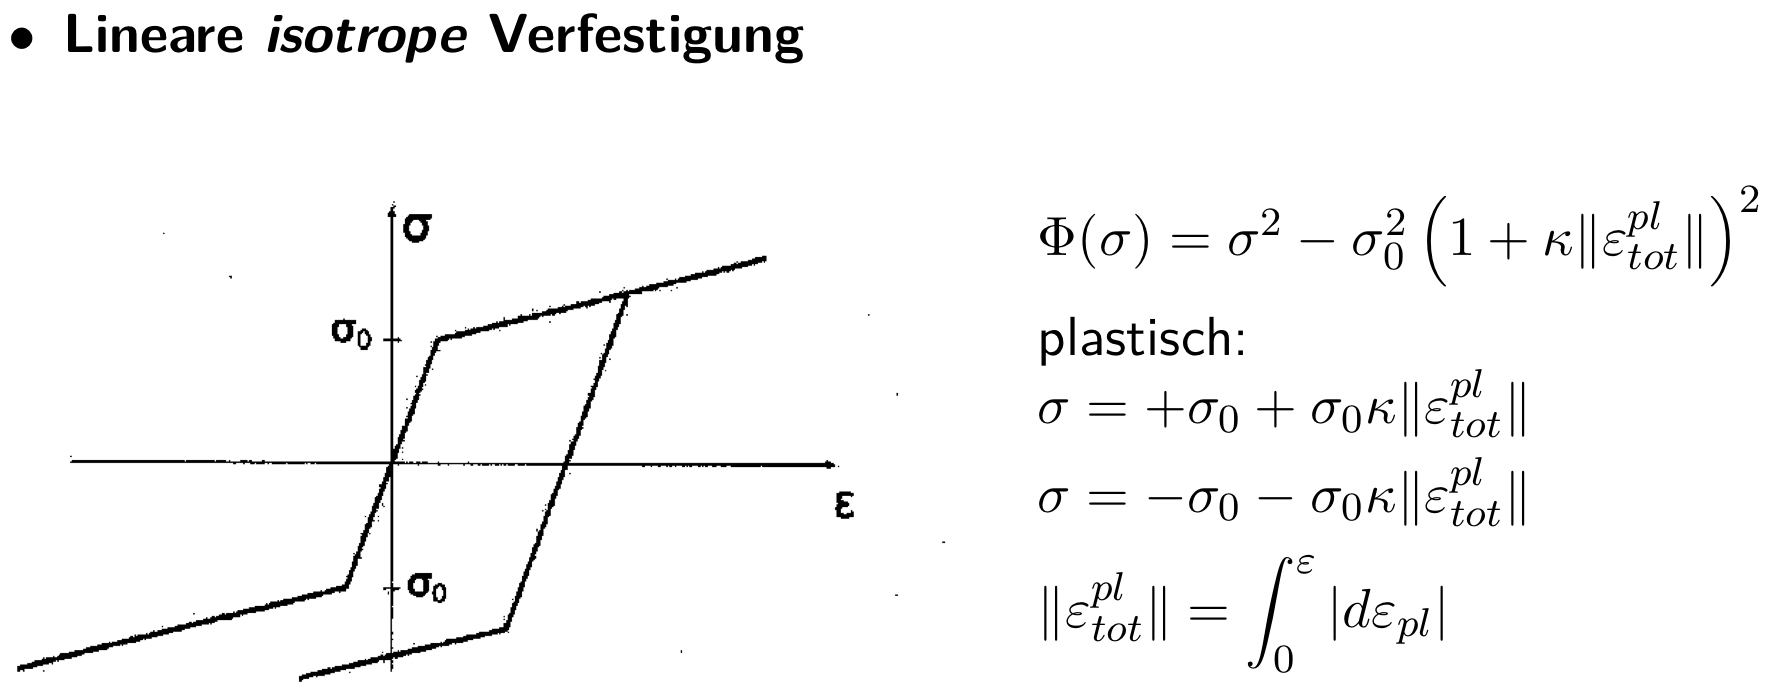
\includegraphics[width=0.5\linewidth]{04/Verf_lin_isotr}
            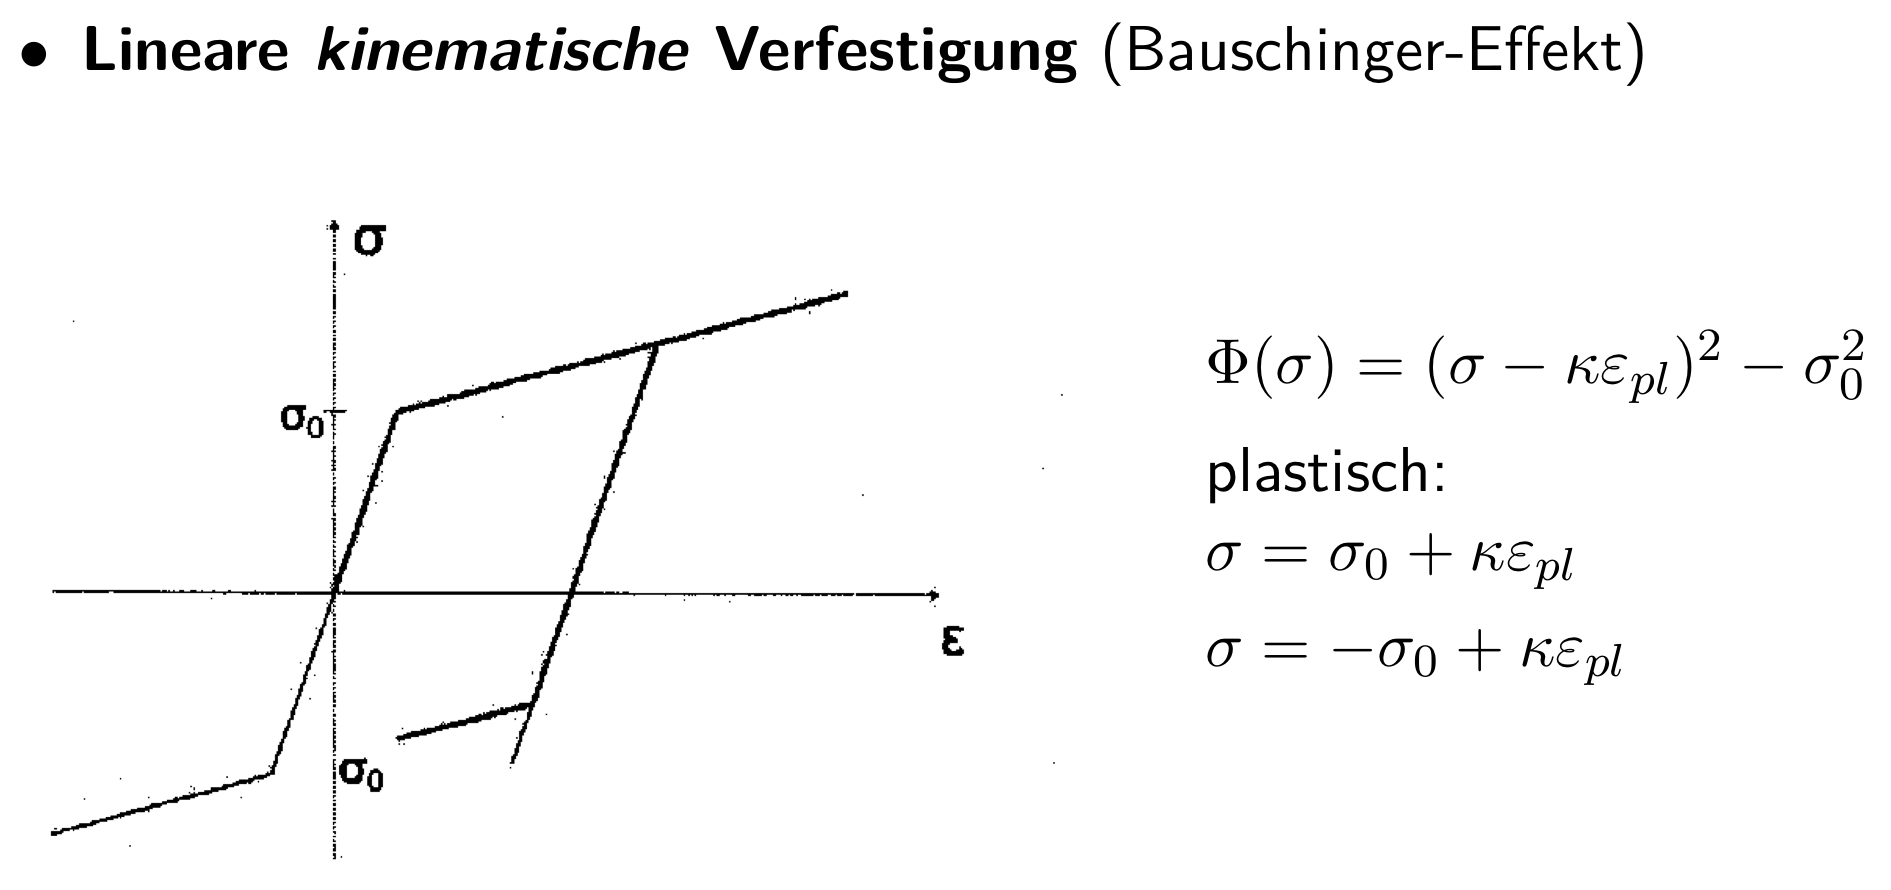
\includegraphics[width=0.5\linewidth]{04/Verf_lin_kin}
        \subsubsection{von Mieses'sche Vergleichsspannung}
            \vspace{-3mm}
            \[\Phi_{\textrm{v.Mises}}= \sigma_1^2+\sigma_2^2+\sigma_3^2-\sigma_1\sigma_2-\sigma_1\sigma_3-\sigma_2\sigma_3 -\sigma_0^2\quad(=0)\]
            \[\Leftrightarrow \sigma_{\textrm{v. Mises}}^{vgl}= \sqrt{\sigma_1^2+\sigma_2^2+\sigma_3^2-\sigma_1\sigma_2-\sigma_1\sigma_3-\sigma_2\sigma_3} \quad\textrm(HS)\]
        \subsubsection{Tresca'sche Vergleichsspannung}
            \textbf{Konservativer als von Mises'sche Vergleichsspannung} (Grenzfläche von Sechseck schneller erreicht als von Ellipse).
            \[\sigma_{\textrm{Tresca}}^{vgl}=\frac{1}{2}\textrm{max} \left(|\sigma_1-\sigma_2|,|\sigma_2-\sigma_3|,|\sigma_3-\sigma_1| \right) =\tau_0=\frac{\sigma_0}{2}\]
    \subsection{Statische Belastung}
        
            % \subsubsection{Kraft- \& Deformationsgesteurete Belastung:}
            % $\frac{\varepsilon_b}{\varepsilon_0}$ Deformationsgesteurete Belastung. Bsp vorgespannte Schraube, therm Spannungen. Begrenzung weniger konservativ $\sigma\varepsilon$-Diagramm gr Dehnung führt zu nur kl Spannungserhöhung).\\ $\frac{\sigma_B}{\sigma_0}$ Kraftgesteuerte Belastung. (Für viele Metalle $\frac{\varepsilon_b}{\varepsilon_0} \gg \frac{\sigma_B}{\sigma_0}$) Überschreiten $R_{p0.2}$ weniger Reserve.
        
        \subsubsection{Spannungsverteilung}
            Falls homogen: bei Fliessgrenze wird die ganze Struktur plastifiziert. $\rightarrow$ Versagen %bei Erreichen der Fliessgrenze wird es in der ganzen Struktur zur Plastifizierung kommen. 
              
            Falls linear: es kommt an lokalen Stellen zu Plastifizierungen $\rightarrow$ Versagen erst bei einer grösseren Belastung.\\
            \textbf{Zug:}
            \begin{itemize}
                \item Erste plastifizierung = vollständige Plastifizierung:
            \end{itemize}
            \[F_{plast} = \sigma_0\ \cdot A\]
            
            %\columnbreak
            \textbf{Biegung:}
            \begin{itemize}
                \item Erste Plastifizierung:
            \end{itemize}
            \[M_{plast} = \sigma_0\cdot I\cdot\frac{1}{y_{\textrm{max}}} \quad\textrm{(mit bspw $\sigma_0 = R_p$)}\]
            \begin{itemize}
                \item Vollständige Plastifizierung:
            \end{itemize}
            \[M_{versagen} = 2\int_{-b/2}^{b/2}\int_{0}^{h/2}\sigma(y)ydydz \quad\textrm{mit $\sigma(y) = \sigma_0$}\]
            
        %\columnbreak
        \subsubsection{Formfaktoren}
            Zug(homogen): $\frac{F_{versagen}}{F_{plast}}$\\
            Biegung(linear): $\frac{P_{versagen}}{P_{plast}}$ (Reserve, da Plastifizierung linear)
    
            

\vspace{-2mm}
\section{FKM Richtlinien}{}
    \subsection{Auslastungsgrad}

        \subsubsection{Definitionen}
            \begin{enumerate}[noitemsep]
                \item $\sigma_{v}$: Vergleichsspannung im Nachweispunkt
                \item $\sigma_{SK}$: Materialfestgkeit, bauteilspezifisch
                \item $J_{ges}$: Sicherheitsfaktor (Gesamtsicherheitsfaktor)
            \end{enumerate}
            \vspace{-1mm}\[\boxed{a_{SK} = \frac{\sigma_{v}}{\sigma_{sk}/J_{ges}}}\]

        \subsubsection{Mehrachsigkeit}
            Falls $h > 1.33$ zusätzlicher Nachweis erforderlich! (Bruchdehnung und ev. maximale äquivalente Spannung bei starker Mehrachsigkeit kleiner)
            \vspace{-2mm}\[\boxed{h = \frac{\frac{1}{3} \textrm{Spur}[T]}{\sigma_{\textrm{v. Mises}}}} \quad \textrm{[T]: Spannungstensor}\]
        \subsubsection{Bauteilfestigkeit $\sigma_{\textrm{SK}}$}
            An Normprobe gemessene Fliessgrenze erffordert meistens Korrektur! \\$R_P$: Fliessgrenze Bauteil; $R_{P,N}$: Fliessgrenze Normprobe.
            \[\boxed{\sigma_\textrm{SK}=R_p\cdot n_{\textrm{pl}}}\]
            \[R_P = K_{d,P}\cdot K_A\cdot R_{P,N};\qquad n_{\textrm{pl}}=\textrm{min} \left( \sqrt{ \frac{E\cdot\varepsilon_{\textrm{ertr}}}{R_p}};K_p \right)\]
            Hom. Spannungsverteilung: $n_{\textrm{pl}}=1$ (Keine Reserve)
            \vspace{-1mm}
            \[\textrm{pl. Formzahl}: \boxed{K_p  = \frac{\textrm{Last beim Versagen
            (zB: }\sigma_{\textrm{v. Mises}}^{vgl}=R_e\textrm{)}}{\textrm{Last bei erster Plast}}}\]
            vollpl.: aus FE; el. Grenzl.: wenn $\sigma_v = R_p$ erreicht.
        \subsubsection{Sicherheitsfaktor $J_{\textrm{ges}}$}
        \small\[J_{\textrm{ges}}= J_s \cdot \left[ J_z \cdot \textrm{max}\left(\frac{J_m \cdot R_p}{R_m}; J_p \right) \right] \]\normalsize
        $J_s$: Lastfaktor (Sicher:=1); $J_z$: Schweissteile; $J_p$: plastifizierung
        \begin{center}
            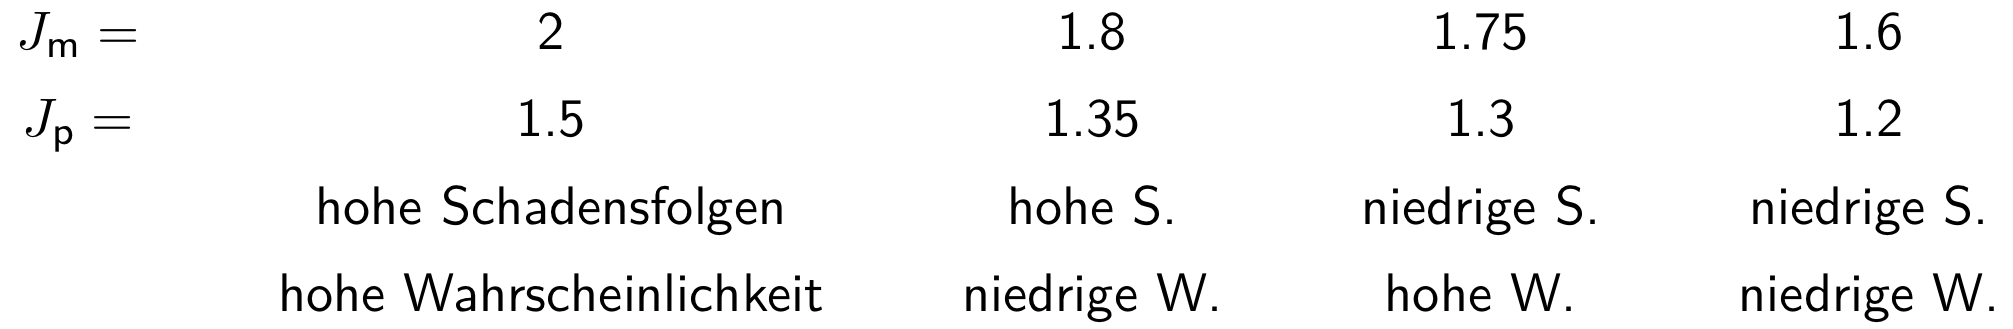
\includegraphics[width=0.8\linewidth]{05/Sicherheitsfaktoren.png}
        \end{center}

    \subsection{Bsp}
        \subsubsection{plastische Formzahl an einem Druckkessel mit Loch}
            \begin{enumerate}
                \item Loch belastet mit $2s,s$ wobei $s=\sigma_{zz}$ $\rightarrow$ kritische Stelle $=5s$
                \item $R_e=5s=5\sigma_{zz}=\frac{5R}{2d}P \Leftrightarrow P_{pl}=\frac{2d}{5R}R_e=:$Last bei erster Plast.
                \item Versagenslast: $R_e=\sigma_{v.Mises}^{vgl}(\sigma_{rr},\sigma_{\varphi\varphi},\sigma_{zz})=\frac{\sqrt{3}R}{2d}R_e \Leftrightarrow P_{vers}=\frac{2d}{\sqrt{3}R}R_e$
                \item $K_p=\frac{P_{vers}}{P_{pl}}\approx 2.88$
            \end{enumerate}

        \subsubsection{Dimensionieren eines Kessels mit Loch nach FKM}
        \textit{Vorgehen:}
        \begin{enumerate}
            \item $ a_{{SK}} = \frac{\frac{\sigma_v}{\sigma_{{SK}}}}{J_{ges}}  \rightarrow  \sigma_v \cdot J_{ges} < \sigma_{{SK}} $
            \item Wegen Mehrachsigkeit kein weiterer Nachweis nötig
            $ h = \frac{1}{3} < 1.33$
            \item Bauteilspezifische Materialfestigkeit $ \sigma_{SK} $ berechnen:
            \item Sicherheitsfaktor $J_{ges}$ berechnen
            \item Einsetzen in 1. ergibt $a_{SK}=0.4<1$
        \end{enumerate}


\section{Zyklische Belastung}
    \subsection{Ermüdung}
        Progressive \textbf{Schädigung durch zyklische Belastung} $\rightarrow$ Riss $\rightarrow$ Dauerbruch\\
        Einflüsse: 3D Spannungszustand, Temp., Korr., Zeit, Frequenz d Zyklen, Kerbwirkung, Mittelspannung, Eigenspannungen, Kumulative Ermüdung, Oberfläche
%\columnbreak
        \subsubsection{Allgemeines Vorgehen}
            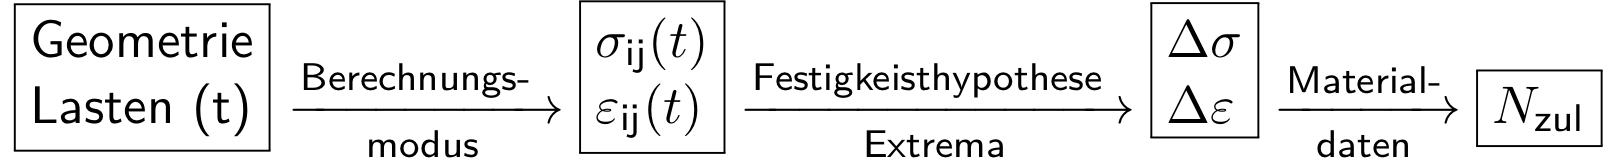
\includegraphics[width=\linewidth]{06/allg_vorgehen.jpeg}
            \vspace{-4mm}
        \subsection{Dauer- \& Zeitfestigkeit}
            \begin{minipage}{\linewidth}
                \begin{itemize}
                    \item bis $10^3-10^4$ Zyklen: \textbf{LCF} (low cycle fatigue - Kurzzeitfestigkeit)
                    \item $10^3-10^4$ bis $10^6$: \textbf{HCF} (high cycle fatigue - Langzeitfestigkeit)
                    \item ab $10^6-10^7$: \textbf{Dauerfestigkeit} - $\sigma_W$: Wechselfestigkeit
                \end{itemize}
            \end{minipage}
%\vfill\null\columnbreak
    \subsection{Einfluss der Mittelspannung auf Dauerfestigkeit}
        \[\sigma_m=\frac{\sigma_u+\sigma_o}{2}; \quad R=\frac{\sigma_u}{\sigma_o} \quad \sigma_m \uparrow, R \uparrow (\sigma_o >0) \rightarrow N_{zul} \downarrow\]
%\vfill\null\columnbreak
        \begin{center}
            \vspace{-1mm}
            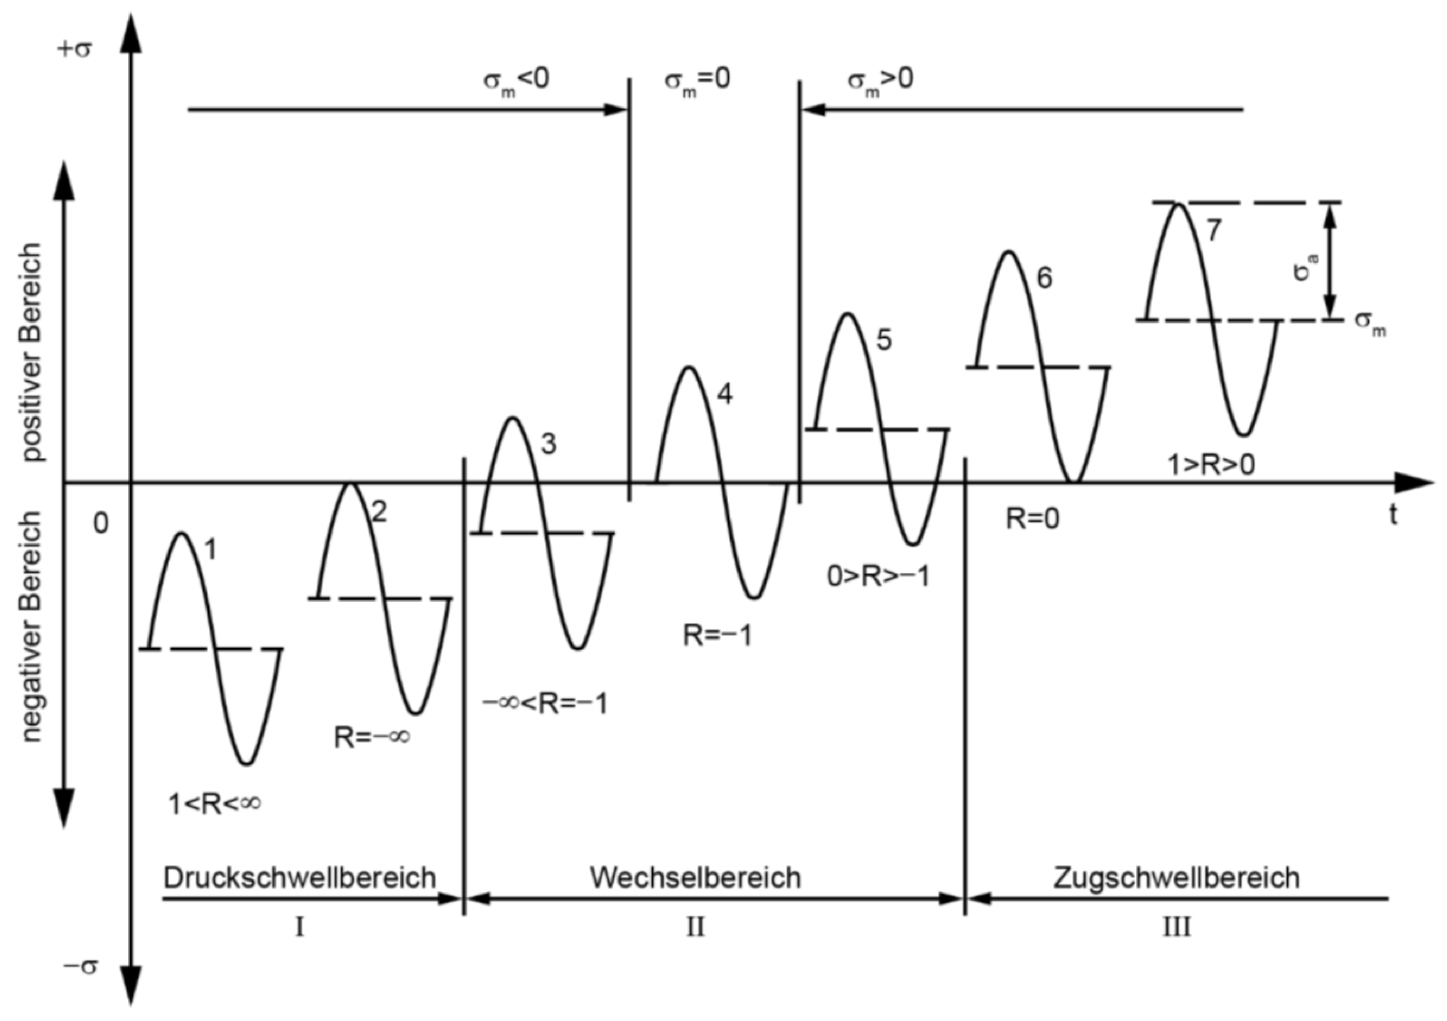
\includegraphics[width=0.7\linewidth, height= 30mm]{06/Einfluss_mittelspannung.png}
        \end{center}
    \subsection{Smith-Diagram}
        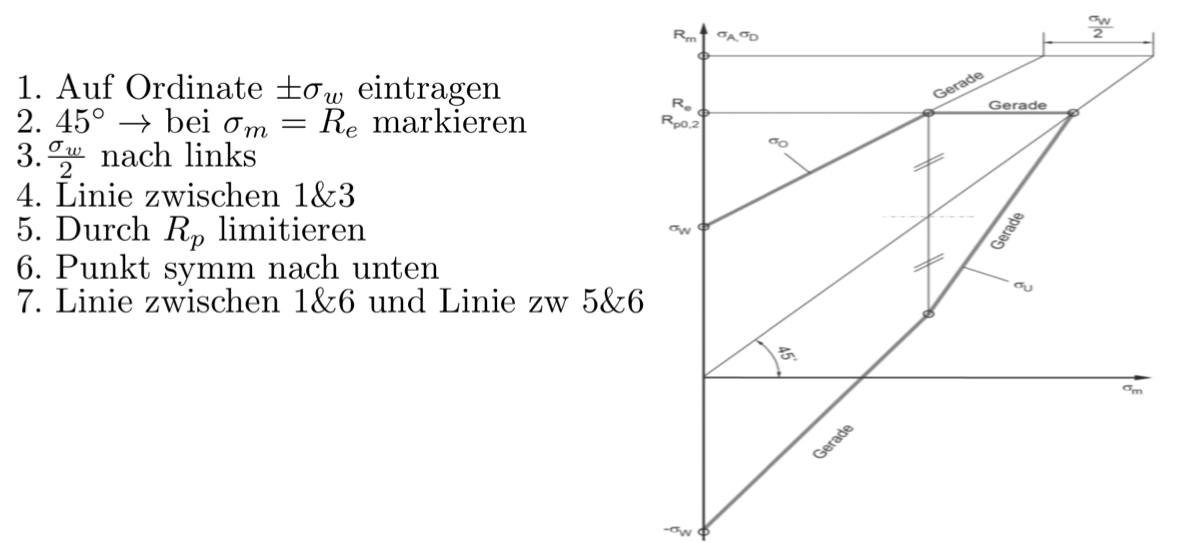
\includegraphics[width=\linewidth, height= 40mm]{06/smith_diagramm.jpeg}
        \vspace{-4mm}
    \subsection{Kumulative Ermüdung (Miner-Regel)}
        Belastung oft komplexer als 'einstufig' $\rightarrow$ Mehrstufenkollektiv. Belastungsfunktion wird in Abschnitte aufgeteilt.
        \vspace{-2mm}
        \[D_{\textrm{BK}}= \sum_{i}\frac{n_{i}}{N_{\textrm{Zul}}(\Delta\sigma_{i},\sigma_{m,i})} \quad D_{\textrm{BK}}: \frac{\textrm{Schädigung}}{\textrm{Belastungskollektive}} \]
        \vspace{-4mm}
        \[T_{L}=\frac{1}{D_{\textrm{BK}}}\cdot T_{\textrm{BK}} \qquad\quad T_{\textrm{BK}}:\frac{\textrm{Belastungszeit}}{\textrm{Belastungskollektive}}\]
\vspace{-2mm}
    \subsection{Kerben}
        \subsubsection{Lokal Elastisch}
            Anriss erfolgt oft an Kerben. An den kritischen Stellen herrscht oft ein \textbf{Ebener Spannungszustand} (Spannungsfreie Oberfläche).\\ $K_F$: Abminderung der Zeitfestigkeit; $K_T$: Abminderung der Wechselfestigkeit. Da $K_F < K_T$ wäre eine Beurteilung basierend auf der lokalen Spannungsamplitude mit der Wöhlerkurve aus ungekerbten Proben zu konservativ. $\sigma_{\textrm{max}}=K_F \cdot \sigma_{\textrm{nom}}$ statt $K_T$.
            \vspace{-2mm}
            \[K_F = q\cdot(K_T-1)+1\]
\vspace{-4mm}
        \subsubsection{Lokal inelastisch (LCF an Kerbe)}
            \vspace{-1mm}
            \[\Delta\sigma_K = K_{\sigma} \cdot \Delta\textrm{s} \qquad \Delta\textrm{s}:\textrm{Fernfeld Schwingbreite}\]
            \[\Delta\varepsilon_K = K_{\varepsilon} \cdot \Delta\textrm{e} \qquad \Delta\sigma_K:\textrm{lok. Schwingbreite}\]
            \[\Delta\textrm{e}=\frac{\Delta s}{E} \qquad\qquad \Delta\varepsilon_K:\textrm{lok. Schwingbreite}\]
    \subsection{Neuber Hyperbel}
        Möglichkeit zur Abschätzung von Dehnungsamplituden bei lokaler plast. im Kerbgrund.
        \vspace{-3mm}\[\sigma_A^E\cdot\varepsilon_A^E = \sigma_A^P \cdot \varepsilon_A^P\]
        \vspace{-2mm}
        Neuber setzt voraus, dass:
        \begin{itemize}
            \item Im Kerbgrund ein einachsiger Spannungszustand besteht.
            \item $\sigma_a^E$ bekannt ( aus finiten Elementen, oder Kerbfaktor)
        \end{itemize}
        \begin{center}
            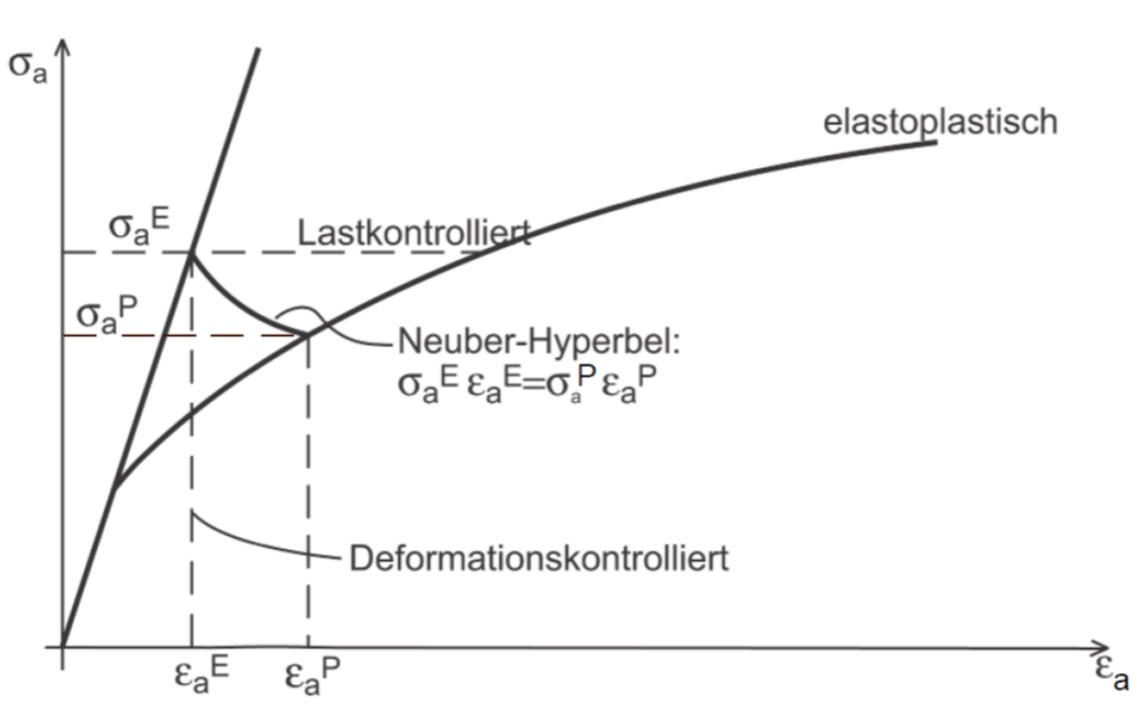
\includegraphics[width=0.7\linewidth, height=30mm]{images/06/Neuber_Hyperbel.jpeg}
        \end{center}{}
        \vspace{-3mm}\[\sigma_a^E = K_T \cdot s; \quad \sigma_a^E = E \cdot \varepsilon_a^E \quad\Rightarrow\quad \varepsilon_a^E = K_T \cdot \frac{s}{E}\]
        \vspace{-4mm}\[\varepsilon_a^P \cdot R_{e}^{zykl.} = K_T^2 \cdot \frac{s^2}{E}; \quad K_{\sigma}=\frac{R_{e}^{zykl.}}{s_a} \quad\Rightarrow\quad K_{\sigma} \cdot K_{\varepsilon} = K_T^2\]
        Falls ideal plastisches Material: (\bm{$\sigma_a^P = \textrm{\textbf{const.}} = R_e^{zykl.}$})
        \\Nützliche Beziehung: $\Delta\varepsilon = 2\varepsilon_{a}^{p}$
    
    

\section{Ermüdung mit örtlichen Spannungen(FKM Kap. 3)}
    \subsection{Lastkollektive Bilden}
    Aus elast. FEM Hauptspannungen an den kritischen Stellen bestimmen.
    aus $\sigma_1(t)-t$ Diagramm Belastungskollektiven einteilen. $\rightarrow \sigma_{1a,1}, \sigma_{1m,1}$; $\sigma_{1a,i}, \sigma_{1m,i}$ bestimmen.
    \\1. Subskript: Welche HS-Richtung (index tiefer $\rightarrow$ HS höher); 
    \\2. Subskript: Welches Kollektiv (index tiefer $\rightarrow$ $\sigma_a$ höher)
    \subsection{Ausnutzungsfaktor für jede HS}
        Ziel: $a_{\textrm{BK},i} < 1$ mit $\displaystyle a_{\textrm{BK},i} = \frac{\sigma_{i,a,1}}{\sigma_{\textrm{BK}}/J_D}$; \quad $J_D=J_S\cdot J_F \cdot J_G$ 
        \\Durchführen für alle Hauptspannungen.
        \[a_{\textrm{ges}}=\sqrt{\frac{1}{2}\left((a_{\textrm{BK}_1}^{*}-a_{\textrm{BK}_2}^{*})^{2}+(a_{\textrm{BK}_2}^{*}-a_{\textrm{BK}_3}^{*})^{2}+(a_{\textrm{BK}_3}^{*}-a_{\textrm{BK}_1}^{*})^{2}\right)}\]
        \[a_{BKi}^*=sign(c_{\sigma i})\cdot a_{BKi} \qquad c_{\sigma i}= \sigma_i(t=t_{max})\]
    \subsection{Berechnung von $\sigma_{\textrm{BK}}$}
        \[\sigma_{\textrm{BK}} = K_{\textrm{BK}} \cdot K_{\textrm{AK}} \cdot \frac{1}{K_{\textrm{WK}}} \cdot \sigma_w \]
        \subsubsection{Kerben \& Oberflächen ($\sigma_{WK}\quad2\rightarrow3$)}
            \[K_{\textrm{WK}}=\left(\left[1+\frac{1}{\widetilde{K}_F}\left(\frac{1}{K_R}-1\right)\right]\frac{1}{K_v}\right)\frac{1}{\eta_{\sigma}}\]
            $\widetilde{K}_F$: Rauheitsfaktor;   $K_R$: Sensitivität auf Rauheit bei Kerben;     $K_v$: Randschichtfaktor;   $\eta_{\sigma}$: Stützzahl aus Kerbwirkung
            \\$\sigma_{WK}$ kann grösser sein als $\sigma_W$
            \\$\eta_{\sigma}=1$ ist konservativ aber $K_R=1$ nicht. (Falls Material $q=1$ wählt man $\eta_{\sigma}=1$)
        \subsubsection{Einfluss der Mittelspannung $\sigma_m$ ($\sigma_{AK}\quad3\rightarrow4$)}
            Aus Haigh-Diagramm:
            \[\textrm{Fall 1: }K_{AK,i}=1-M\frac{\sigma_{m,i}}{\sigma_{a,i}}\quad\textrm{Fall 2: }K_{\textrm{AK},i}=\frac{1}{1+M\frac{\sigma_{m,i}}{\sigma_{a,i}}}\]
            $\sigma_{AK}$ immer $\leq\sigma_{WK}$ aber nicht immer $\leq\sigma_W$
        \subsubsection{Beschränkte Schwingungszahl ($\sigma_{BK}\quad4\rightarrow5$)}
            Einstufenkollektiv: $\displaystyle K_{\textrm{BK}}= \frac{\sigma_{a}(N=N_L)}{\sigma_w}$\\
            \[ K_{\textrm{BK}}=\frac{\sigma_{a}^{**}(\bar{N})}{\sigma_{a}(N_{D})}=\frac{c_1\left(\frac{AD_M}{\bar{N}}\right)^{1/K}}{c_1\cdot N_D^{-1/K}}=\left(\frac{A\cdot D_{\textrm{m}}\cdot N_{\textrm{D}}}{\bar{N}}\right)^{1/K}\]
            \[A = \left[\frac{n_1}{\bar{N}}\cdot\left(\frac{\sigma_{a,R,1}}{\sigma_{a,1}}\right)^{K}+\frac{n_2}{\bar{N}}\cdot\left(\frac{\sigma_{a,R,2}}{\sigma_{a,1}}\right)^{K}\right]^{-1}\]
            \[ \sigma_{a,R,i}=\sigma_{a,i}\cdot\frac{K_{\textrm{AK},1}}{K_{\textrm{AK},i}}\]
            
            $\bar{N}$: $\Sigma$ Zyklen; \qquad $D_{\textrm{m}}$: Schadensgrenze $<1$
            
            \[\sigma_{AK}=c\cdot N_D^{-1/K}; \qquad \sigma_{a,1}= c\cdot N_{zul}(\sigma_{a,1})^{-1/k}\]
            \[\Rightarrow \sigma_{AK}= \sigma_{a,1}\left(\frac{N_{zul}}{N_D}\right)^{1/k}\]
            \[N_{zul}(\sigma_{a,R,i})=N_{zul}(\sigma_{a,1})\left(\frac{\sigma_{a,1}}{\sigma_{a,R,i}}\right)^K\]

\vfill\null\columnbreak

\section{Kriechen}
    \subsection{Definiton}
        \begin{itemize}
            \item Inelastische Dehnungen
            \item Für Sekundärkriechen: $\dot{\varepsilon}_{cr} = f(T,\sigma)$;\\$\sigma = \textrm{const.} \Rightarrow \dot{\varepsilon}_{cr}= \textrm{const.}$
        \end{itemize}
        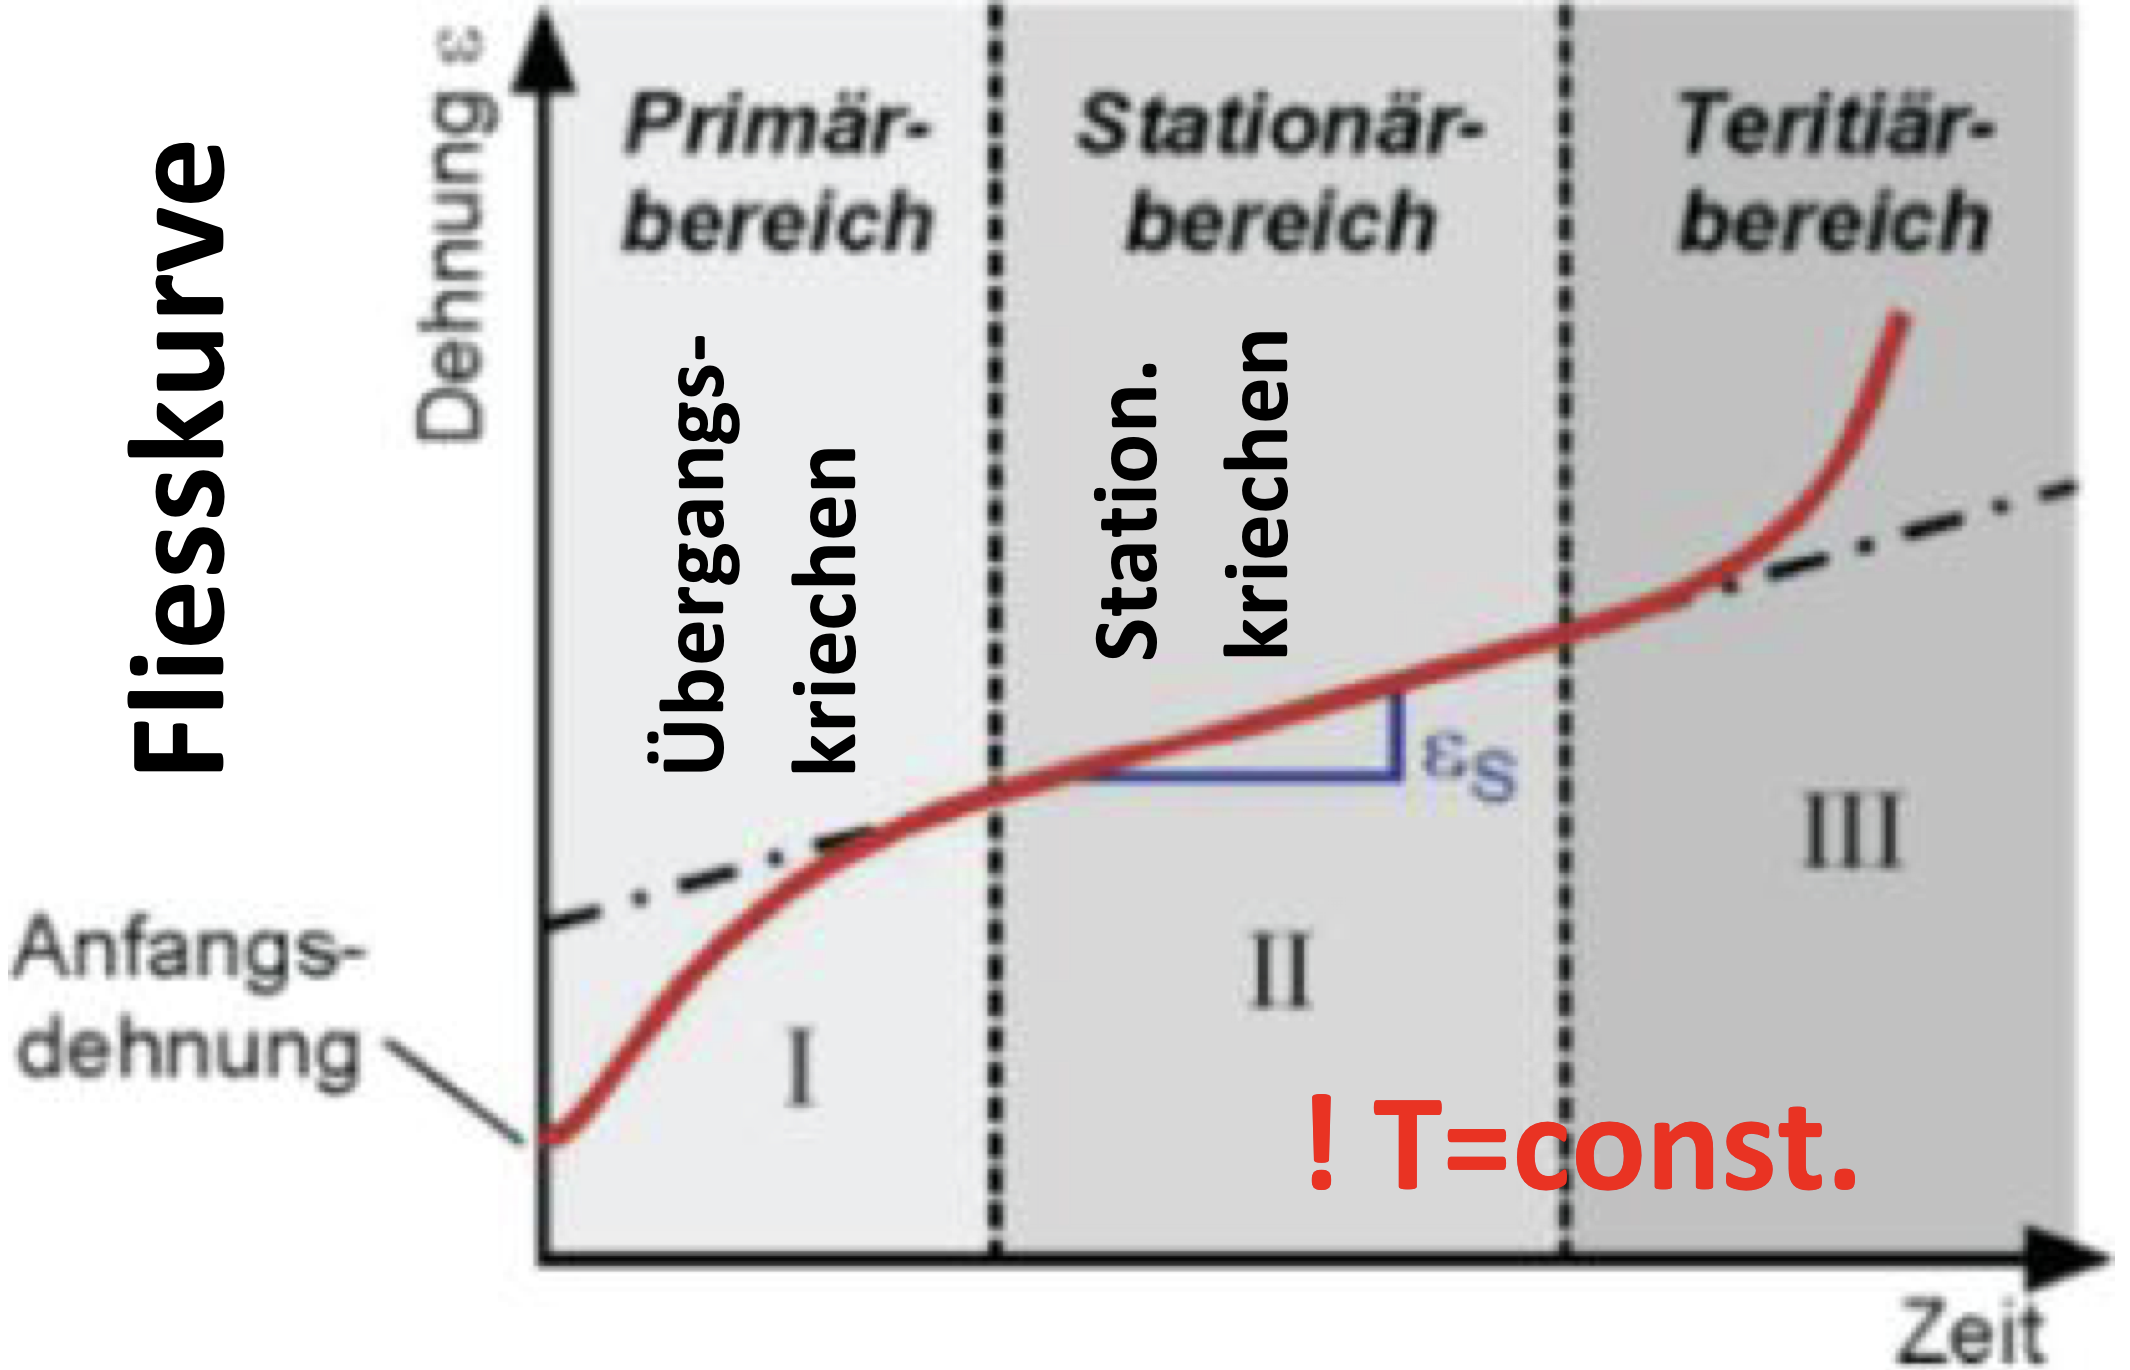
\includegraphics[width=0.45\linewidth]{08/Kriechkurve1.png}
        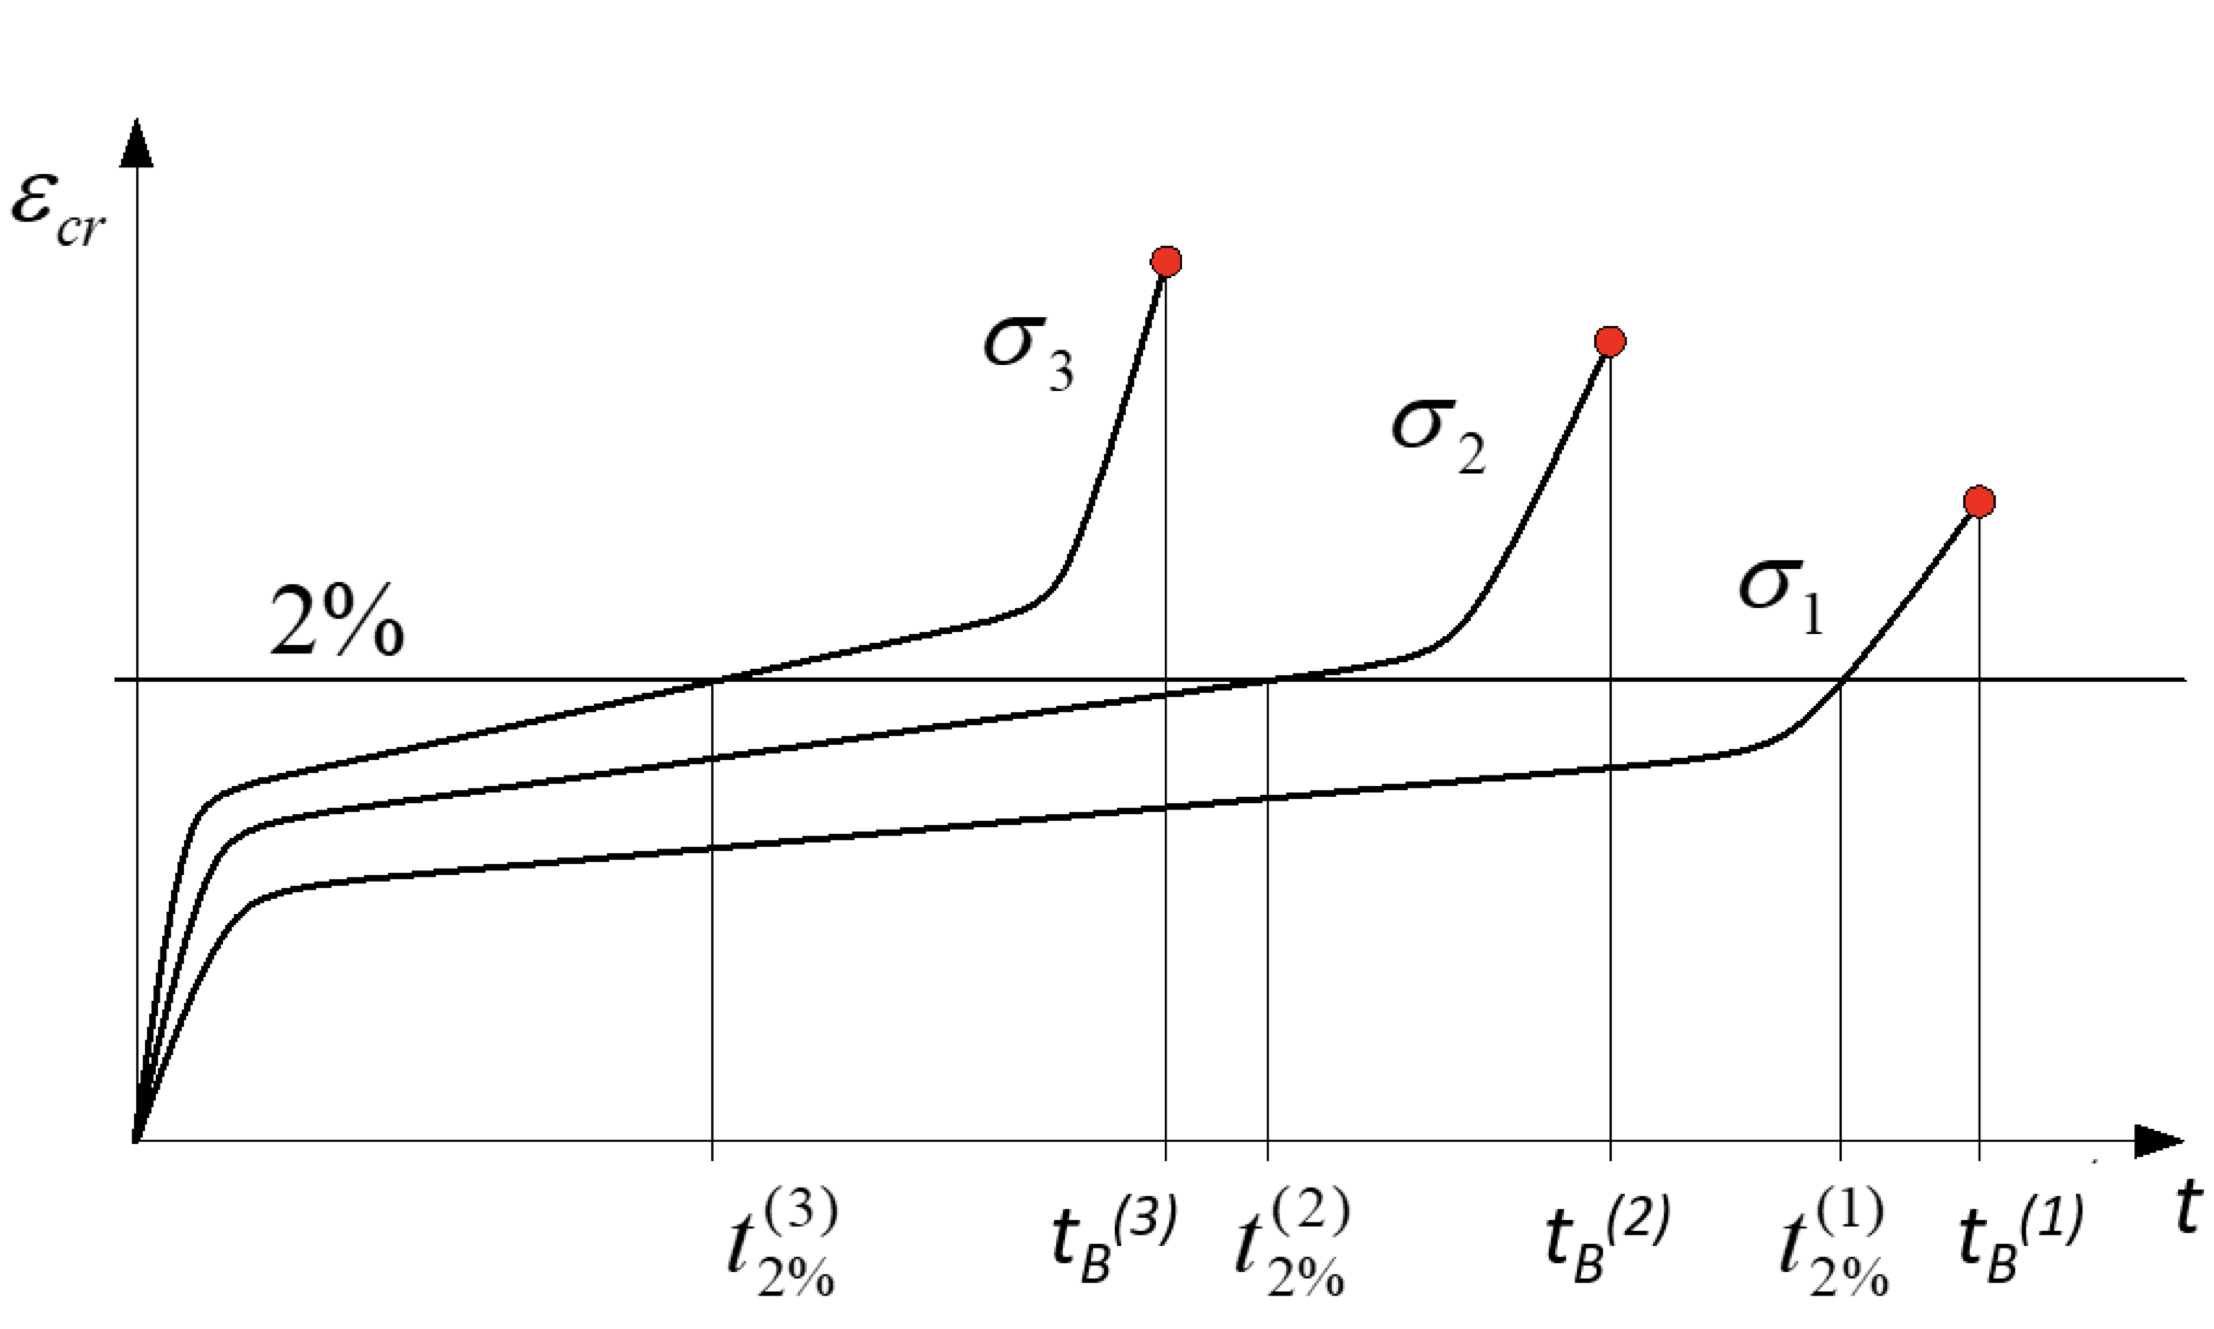
\includegraphics[width=0.55\linewidth, ]{08/E_cr-t-diag.png}
    \subsection{Ursachen}
        Kriechen tritt bei metallischen Stoffen bei $ T > T_{schmelz} \cdot 0.3  $ auf.
        Bewegung von Versetzungen, Gleit- und Diffussionsphänomene. $\rightarrow$ \textbf{inelastische Deformation}
        
    \subsection{Relaxation}
        \subsubsection{Nach Norton}
            %ges: $\sigma(t)$ geg: $\varepsilon_{cr}$, $\varepsilon{el}$
            \[\varepsilon_{cr}+\varepsilon_{el}=\varepsilon_0=\textrm{const.} \qquad \dot{\varepsilon}_{cr}+\dot{\varepsilon}_{el}=0 \Rightarrow A\sigma^n + \frac{\dot{\sigma}}{E}=0\]
            Separation der Variablen und Integrationskonstante mit Anfangsspannung bestimmen.
            \\\textbf{Analytische Lösung:}
            \vspace{-2mm}\[\sigma(t)=\left(\sigma_{0}^{1-n}-(1-n)A\cdot E\cdot t\right)^{\frac{1}{1-n}}\]
%\columnbreak
    \subsection{Kriechschädigung}
        \subsubsection{Kumulative Schädigung/ Time Fraction Rule}
            Spannungsgeschichte $\sigma(t)$ in \textbf{diskrete Intervalle} $\Delta t_n$ mit konstanter Spannung $\sigma_n$ \& zugehöriger Rupture-Time $t_B(\sigma_n)$ aufteilen.
            \vspace{-2mm}\[D_{cr}=\sum_n\frac{\Delta t_{n}}{t_B(\sigma_n)} < 1\]
            \textbf{kontinuierliche Sannungsgeschichte:}
            \vspace{-2mm}\[D_{cr}=\int_0^t\frac{1}{t_B(\sigma(t))}dt < 1\]
            Spannungsrelaxation$\rightarrow \sigma(t)$ mit $\dot{\sigma}<0$
%\columnbreak
        \subsubsection{Ductility Exhaustion Method}
            \[D_{cr}=\int_0^{\bar{\varepsilon}_{cr}}\frac{1}{\varepsilon_{cr}^B(\dot{\varepsilon}_{cr})}d\varepsilon_{cr} \approx \int_0^{\bar{\varepsilon}_{cr}}\frac{\dot{\varepsilon}_{cr}}{\varepsilon_{cr}^B(\dot{\varepsilon}_{cr})}dt< 1\]
            $\bar{\varepsilon}_{cr}$: ersetzen durch $\varepsilon_{cr}(t_{Ende})=\varepsilon_0-\frac{\sigma(t_{Ende})}{E}$
            \\Beobachtung: $\varepsilon_{cr}^{B}\downarrow$ mit zunehmender Hydrostatischer Belast.
        \subsubsection{Lebensdauer}
            \[N\cdot D_{cr}^{BK} = 1\]
            $N$: Anzahl Zyklen bis zu Versagen (siehe Miner Regel)
    \subsection{Interaktion Kriechen-Ermüdung}
        Kriechen oder Relaxation innerhalb einer zyklischen Belastung führen zu niedriger $N_{zul}$ für gleiche Dehnungsschwingbreite $\Delta\varepsilon$. $\qquad D_{cr}\uparrow \quad\rightarrow\quad N_{zul}(\Delta\varepsilon)\downarrow$\\
            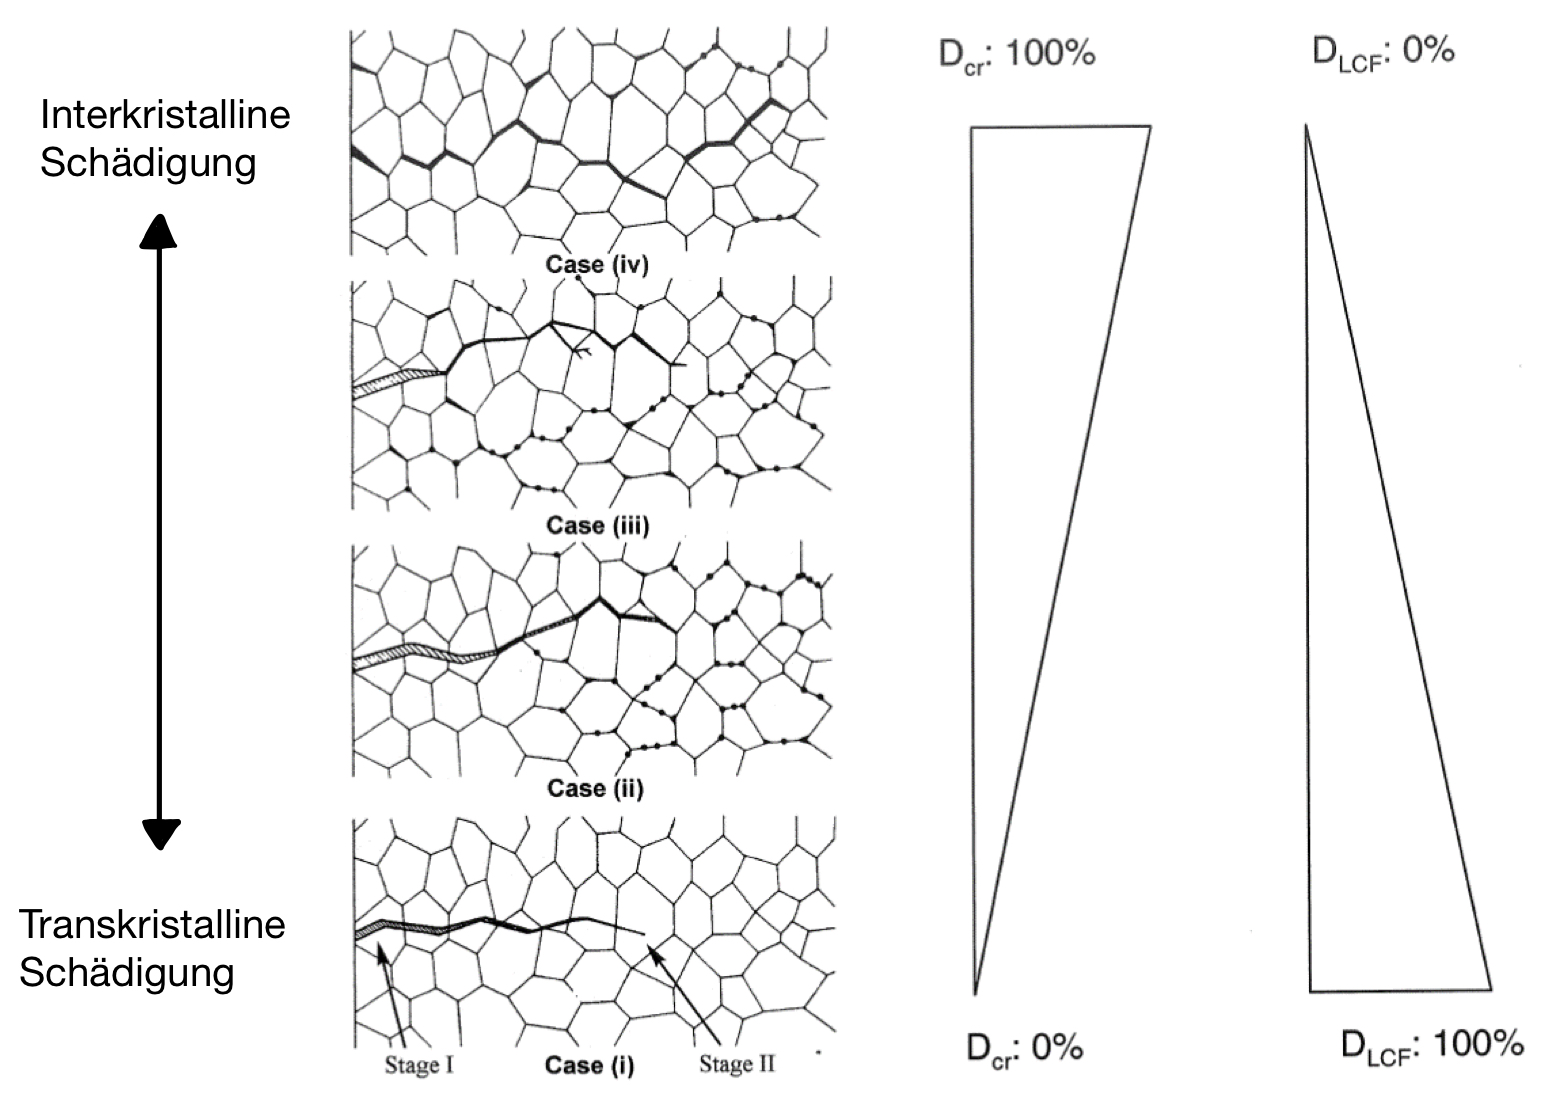
\includegraphics[width=0.55\linewidth, height=30mm]{08/LCF_schaed.jpg}
            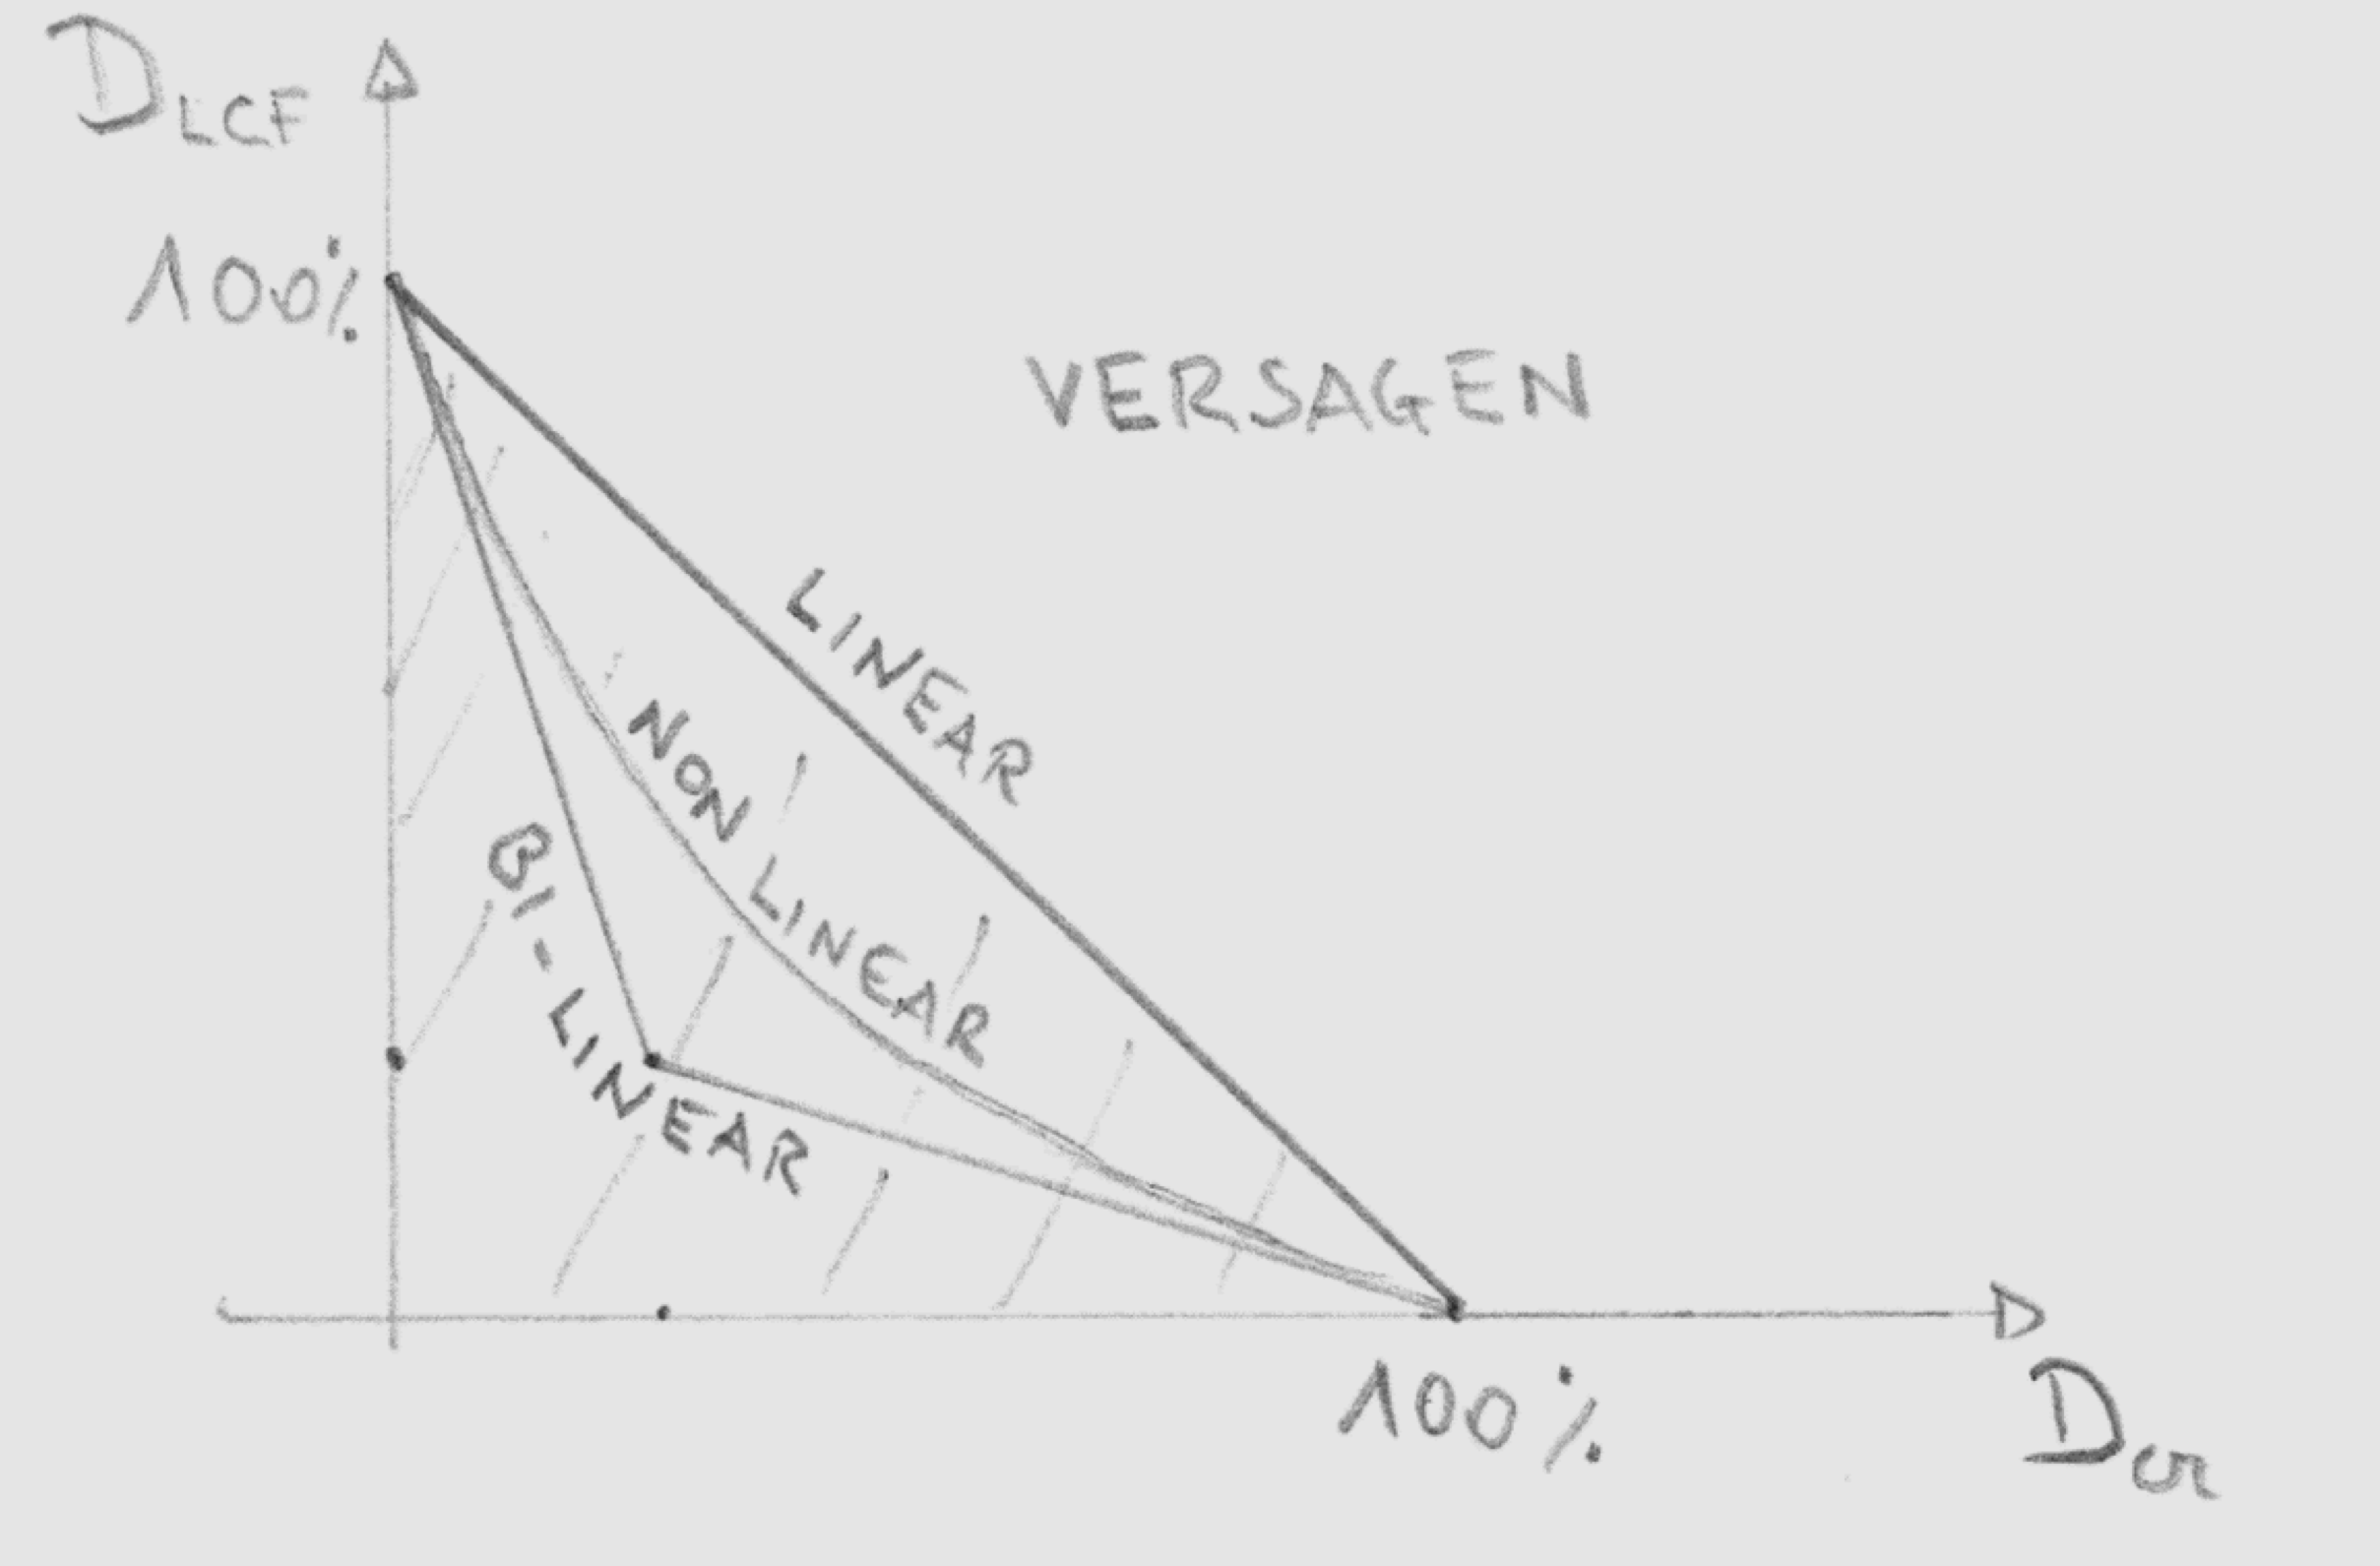
\includegraphics[width=0.45\linewidth, height=30mm]{08/damage_sum_diag.png}
        

\section{Stabilität}
    \subsection{Stabilitätsprobleme}
        Stetiger oder plötzlicher Übergang zu stabilen aber meistens unerwünschten deformierten Zuständen.\vspace{-1mm}
        \begin{itemize}
            \item Bei welcher Last findet der Übergang statt?
            \item Wie sieht das Deformationsbild aus?
        \end{itemize}
        \begin{center}
            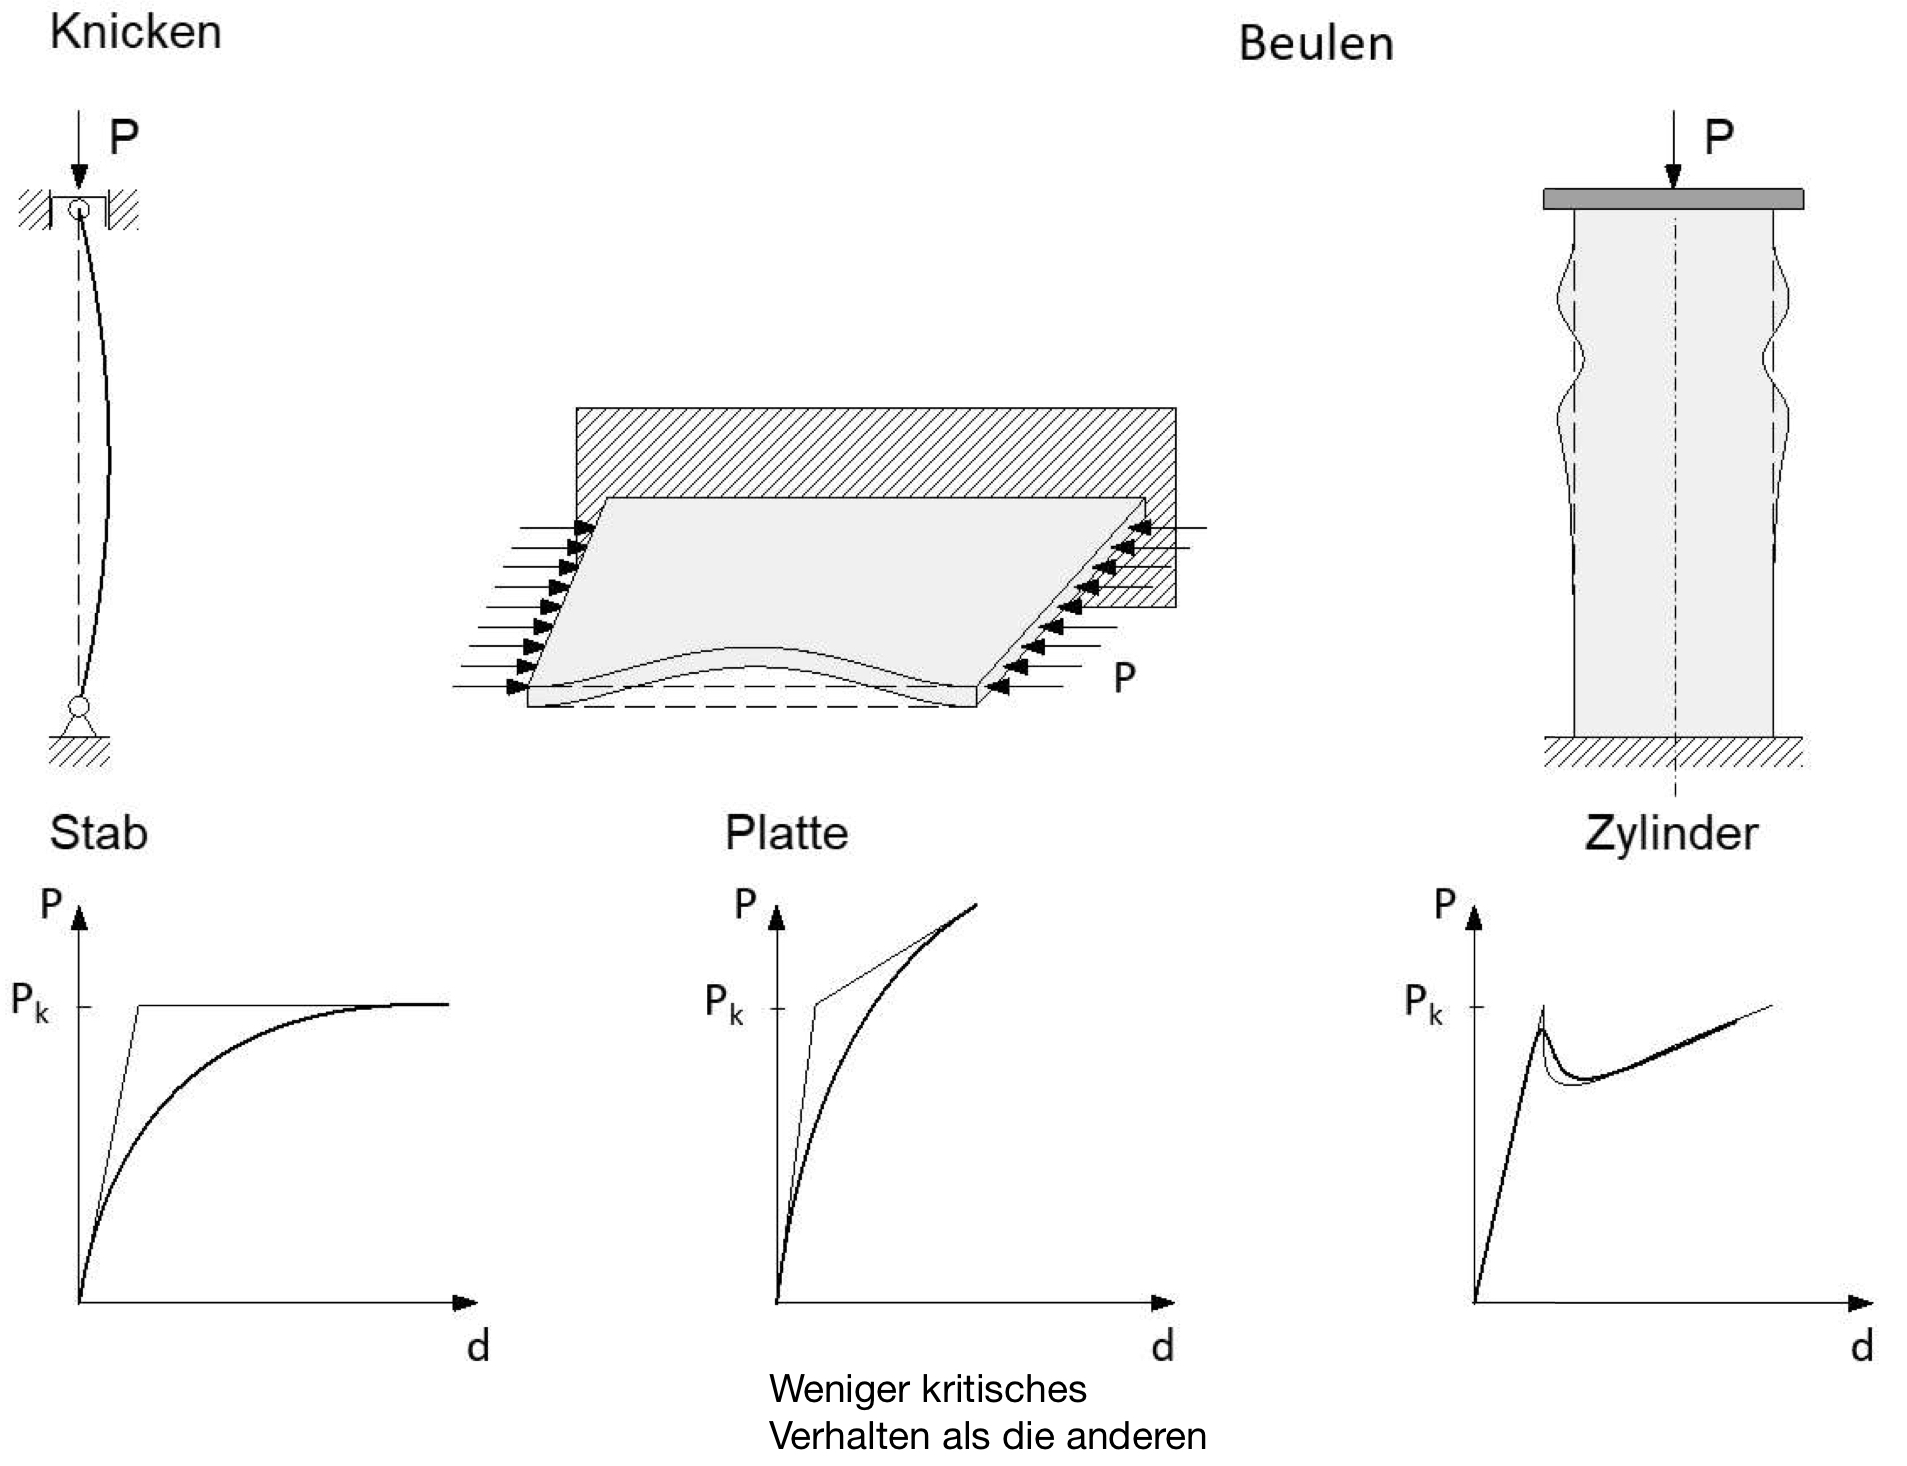
\includegraphics[width=0.7\linewidth , height= 30mm]{09/stability.jpeg}
        \end{center}
    \subsection{1D-Stabilitätsproblem}
        Balken axial belastet, an den Enden axial geführt (oben) und gelenkig gelagert (unten).
        \begin{center}
            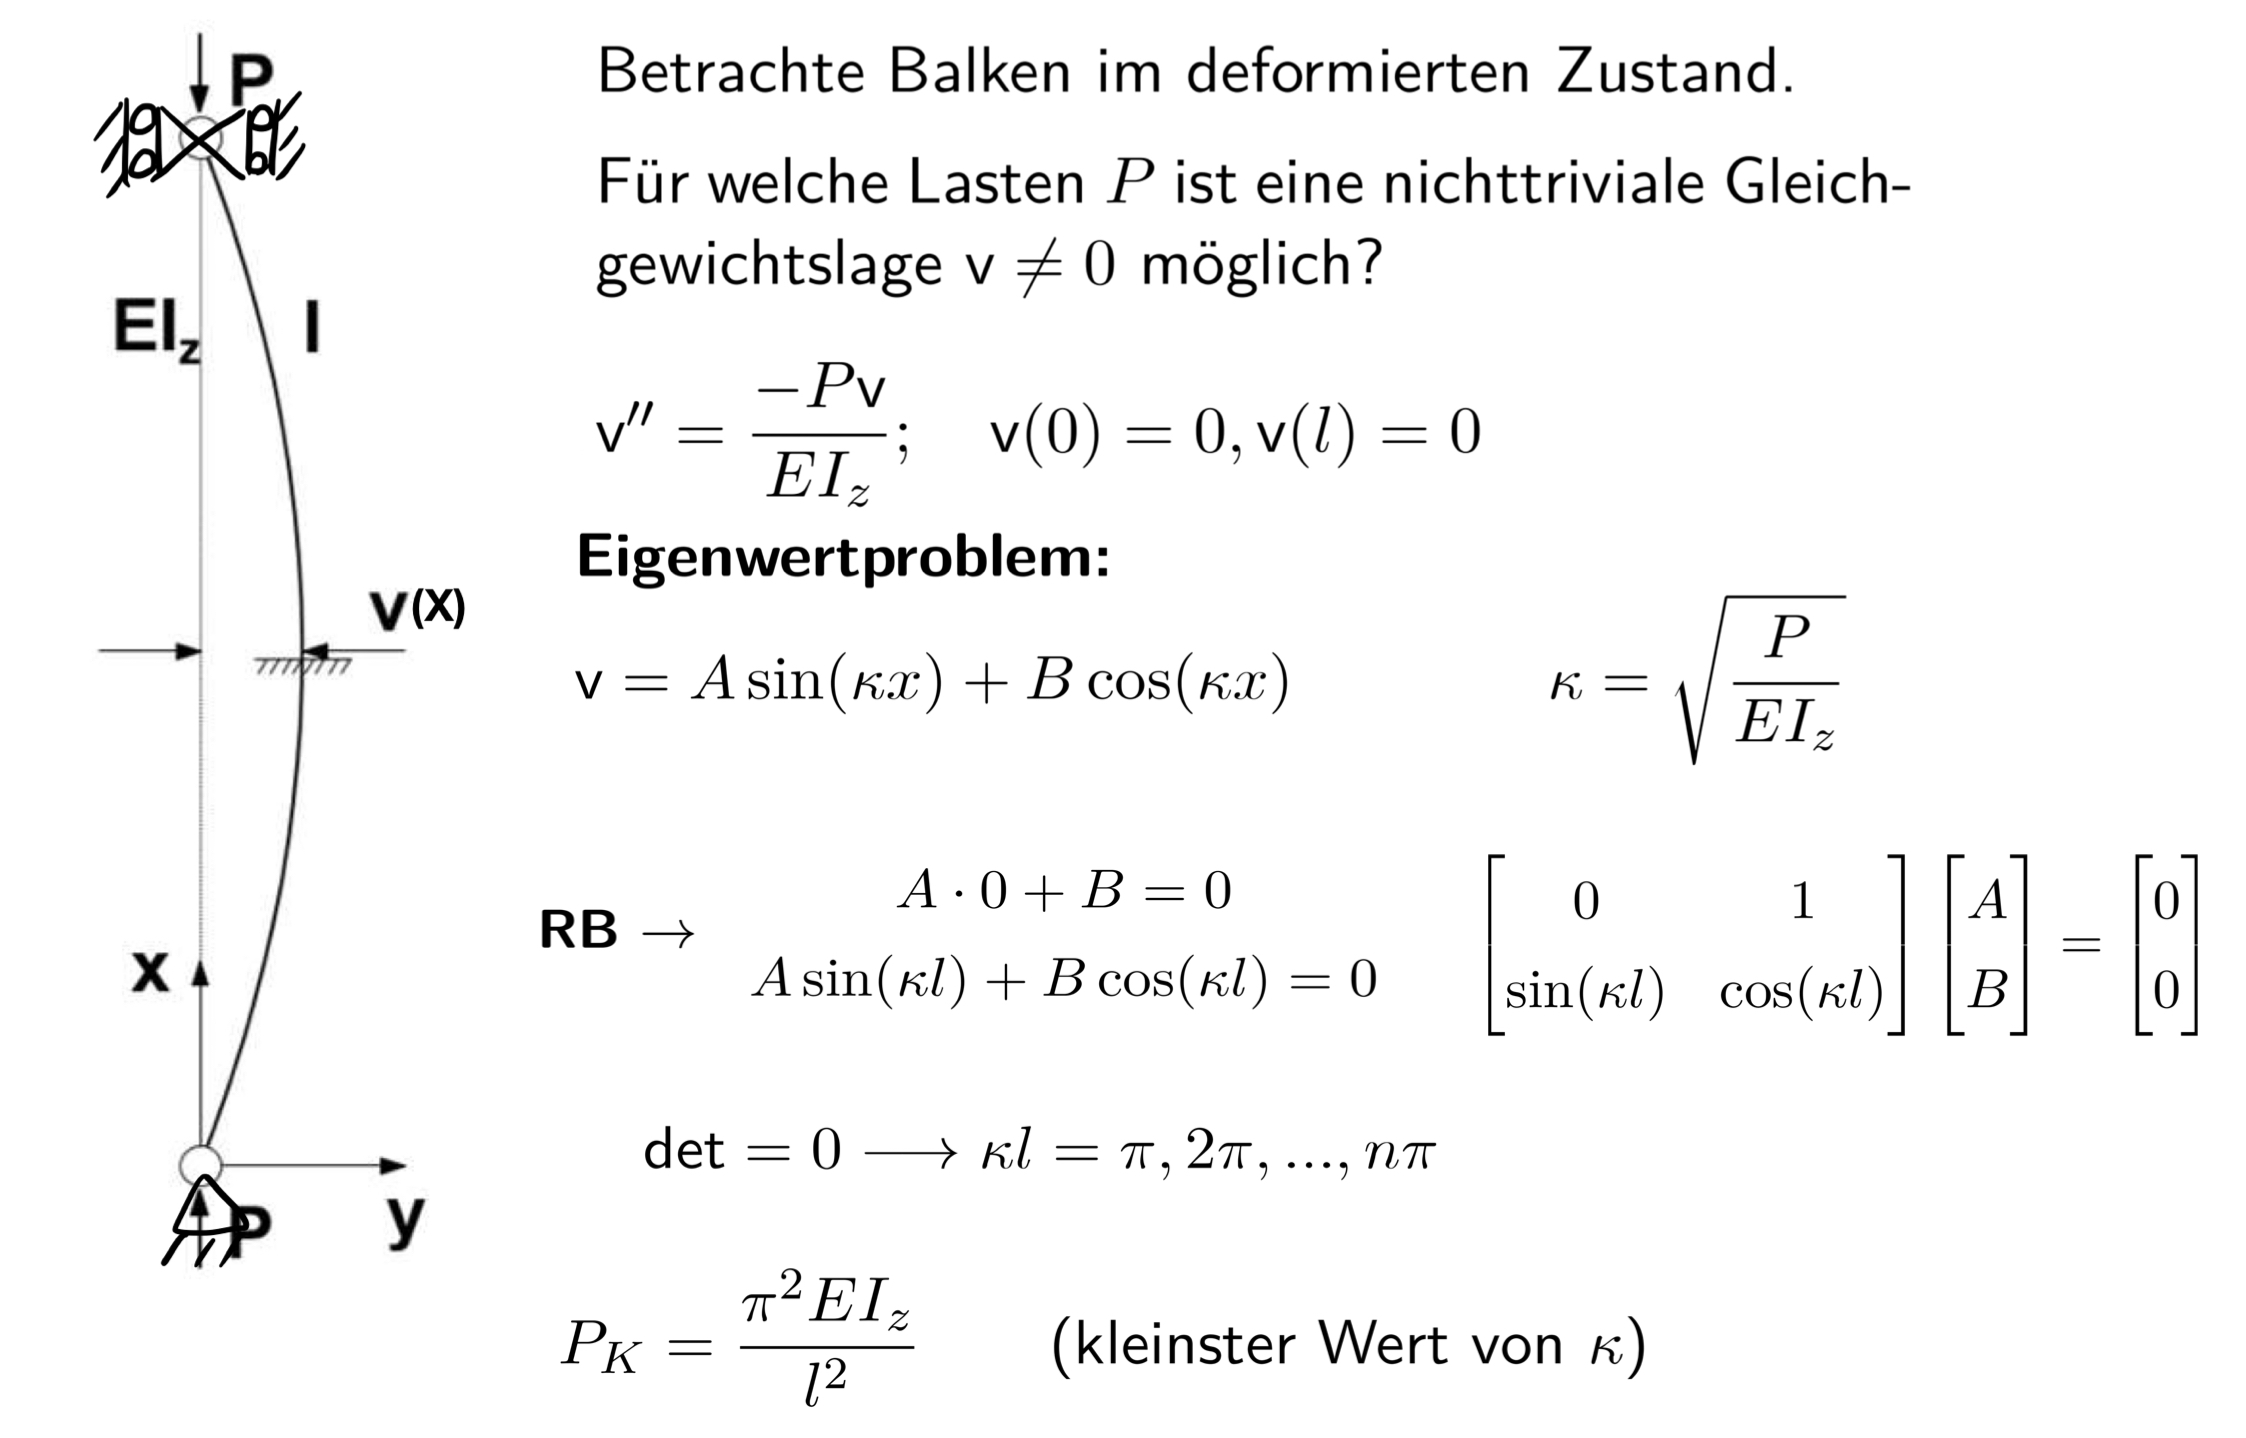
\includegraphics[width=0.9\linewidth,height=45mm]{09/1d.jpeg}
            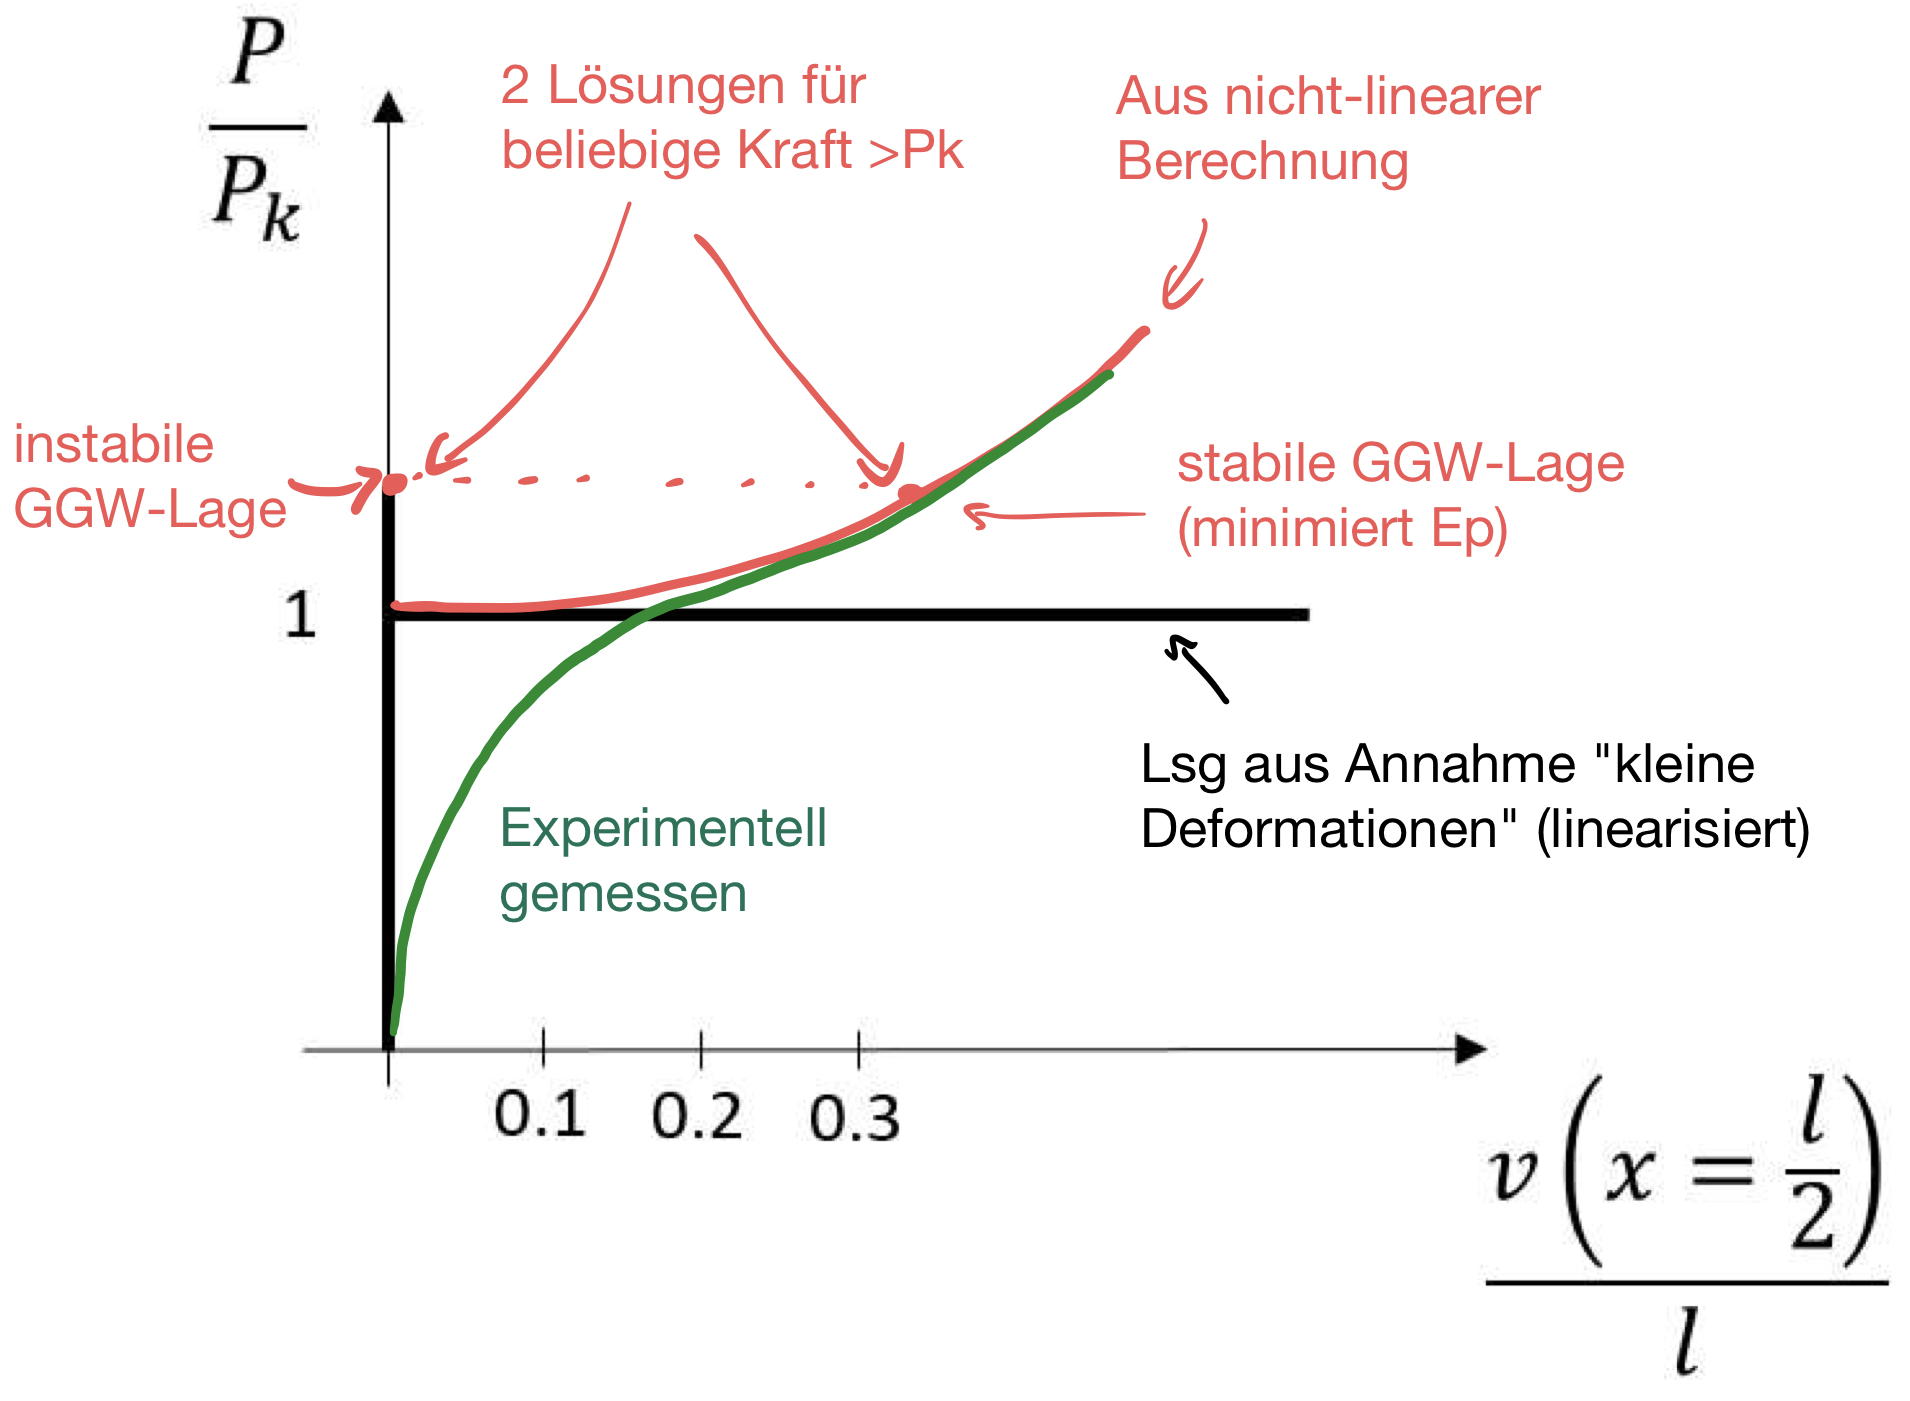
\includegraphics[width=0.85\linewidth, height=45mm]{09/1d-graph.jpeg}
        \end{center}
        Balken einer Seite eingespannt \& andere Seite los.
        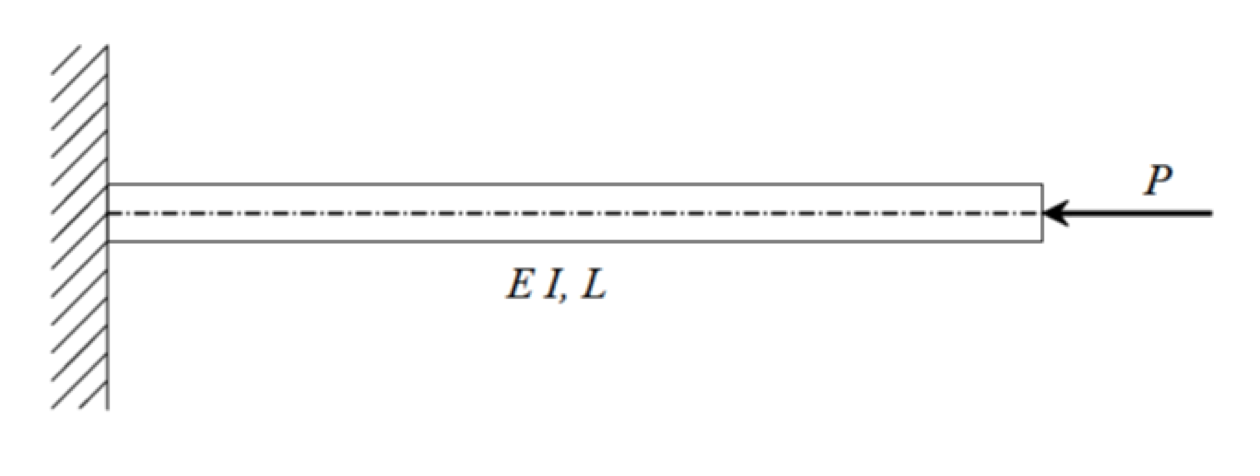
\includegraphics[width=0.6\linewidth]{09/uebung.png}
        \vspace{-17mm}
        \begin{flushright}
        $\displaystyle P_k=\frac{\pi^2EI_z}{4L^2}\qquad\qquad$
        \end{flushright}
        \vspace{7mm}
        
        \begin{comment}
        \subsubsection{Plastifizieren vor Knicken}
            $P_{plast} \leqslant P_k $
        \end{comment}
    \subsection{System mit 1-Freiheitsgrad}
        \TODO{}


\end{multicols*}     

\end{document}